% The following choice requires a coordinated choice when PRINTING the report:
%\documentclass[oneside,12pt]{report}  % Use this for one-sided copying (print with printer's normal
%  single-sided option
\documentclass[twoside,12pt,openright]{report}  % You can use this for a slim final printed copy (print with 
%  printer's double-sided option)

% the dimensions of the page
\textheight=9.25in \topmargin=-0.5in   %See note in Chapter 8 of Sample Report about "Page scaling" option in Adobe
\textwidth=6.0in
\oddsidemargin=0.3in
\evensidemargin=0.3in  % Needed to balance even and odd pages in twoside print copy

% Useful packages
\usepackage{amsmath}
\usepackage{amsfonts}
%% In the following, the assumption is that your graphics are in encapsulated postscript (eps).  If not,
%% you may need to use some other method for incorporating graphics into your pdf of the final report.
%  Use the next package for typesetting directly to dvi or postcript (used primarily for the PCTeX typesetter, 
%  see the following alternatives).
\usepackage[dvips]{graphicx} 
% Use the next two packages together for typesetting directly to pdf (this works for pdfLaTeX and may work 
% for others---not yet tested for all---please report your experience).
%\usepackage[pdftex]{graphicx}
%\usepackage{epstopdf}
%%

\usepackage{doc}
% Following sets up logic and formatting for conditional twoside copying
\usepackage{ifthen, color, fancyvrb}
\usepackage{nextpage}\pagestyle{plain}
\newcommand\myclearpage{\cleartooddpage
  [\thispagestyle{empty}]
  }

%  Set font size for captions
\usepackage[skip=4pt,font=footnotesize]{caption}


\DeclareGraphicsExtensions{ps,eps}
\usepackage{excludeonly}

% If some words are being hyphenated incorrectly, they can be
% given in a list to the \hyphenation command as below.
\hyphenation{ap-pen-dix wer-ther-i-an}

% Theorem-like command definitions:
\newtheorem{theorem}{Theorem}[chapter]
\newtheorem{lemma}{Lemma}[chapter]
\newtheorem{definition}{Definition}  % Note, this italicizes everything

% Print the chapter and sections in the toc
\setcounter{tocdepth}{1}

% Specify which files to typeset for this run (note that overall pagination is preserved)
%\includeonly{chapter1, chapter2}

% Specify which files NOT to typeset for this run (note that overall pagination is preserved)
%\excludeonly{}

% Groundwork for allowing double-sided copying with blank versos
\def\prefacesection#1{
\chapter*{#1}
\addcontentsline{toc}{chapter}{#1}
}

\begin{document}

% Footnote references are symbolized in the front matter, but see below for restoration of numbered footnotes in the body.
\def\thefootnote{\fnsymbol{footnote}}

% The title page is in its own file, ``titlepage.tex''.
% It needs to be edited to reflect information specific
% to your project. 
% don't display the page number
\thispagestyle{empty}

% The numbers below controls the amount of space between the following sections
\def\shiftdowna{0.32in}  % Adjust for balance
\def\shiftdownb{0.22in}  % Adjust for balance

% Set up the boiler plate at the top of the page

\begin{center}
\textbf{{\large Summer Research Program in Industrial \\ and Applied Mathematics}}\\

\vspace \shiftdowna
%\includegraphics[width=0.4\textwidth]{ipam.eps}\\

\begin{figure}[h]
  \centering
  \begin{minipage}[b]{0.4\textwidth}
    \centering
    
\includegraphics[width=3cm]{Graphics/HKUST_logo.jpg}
      \end{minipage}
 % \hfill
  \begin{minipage}[b]{0.4\textwidth}
    \centering
    \includegraphics[width=6cm]{Graphics/SNU_logo.jpg}
      \end{minipage}
\end{figure}

% SPONSOR
\vspace \shiftdowna
\underline {Sponsor}\\ 
\vspace{5pt}
$\langle \textbf{{\large Magnum Research Limited}} \rangle$ \\
\vspace \shiftdowna
\textbf{Final Report}

% TITLE
\vspace \shiftdowna
$\langle \textbf{{\Large Portfolio Management using Reinforcement Learning}}\rangle$

% Note the convention used here:  email addresses and urls are typeset in teletype font, colleges are set in italics.

% STUDENTS
\vspace{0.35in}
\underline {Student Members}\\
\vspace{5pt}
$\langle \text{SEO Dayoung}\rangle$ (Project Manager), $\langle \text{\emph{SNU}}\rangle$,\\ 
\vspace{3pt}
$\langle \text{\texttt{Contact Info}} \rangle$\\
\vspace{5pt}
$\langle \text{PARK Junggil}\rangle$, $\langle \text{\emph{SNU}} \rangle$ \\
\vspace{3pt}
$\langle \text{WONG Singlam}\rangle$, $\langle \text{\emph{HKUST}} \rangle$ \\
\vspace{3pt}
$\langle \text{YANG Yuwei}\rangle$, $\langle \text{\emph{CityU HK}} \rangle$ \\

% ACADEMIC MENTORS
\vspace \shiftdownb
\underline {Academic Mentor} \\
\vspace{5pt}
$\langle \text{Avery Ching}\rangle$, $\langle \text{\texttt{Contact Info}} \rangle$

% SPONSORS
\vspace \shiftdownb
\underline {Sponsoring Mentors}\\
\vspace{5pt}
$\langle \text{Don Huang}\rangle$, $\langle \text{\texttt{Contact Info}} \rangle$\\
\vspace{3pt}
$\langle \text{Joseph Chen}\rangle$, $\langle \text{\texttt{Contact Info}} \rangle$


% DATE
\vspace \shiftdowna
$\langle \text{Date: August 8, 2018}\rangle$ 

\end{center}

%\vfill  %Fill page to force following note to bottom
%\footnoterule
%\noindent \small{This project was jointly supported by HKUST and SNU.} 



% Begin ABSTRACT
\ifthenelse{\boolean{@twoside}}{\myclearpage}{}
\prefacesection{Abstract}
% don't display the page number
%\thispagestyle{empty}

This sample report serves two purposes.
First, it introduces the RIPS ``house style''---preferences for how copy is set and laid out on a page.%%
\footnote{
R. M. Ritter, {\em New Hart's Rules:  The Handbook of Style for Writers and Editors}, Oxford University Press, 2005.
}
Second, by comparing this document with the {\LaTeX} source, it illustrates the effects of {\LaTeX} code on the resulting typeset.%
\footnote{
Location of the source code is provided in Appendix \ref{App:SourceLocation}.
}

\vspace{24pt}
(The Abstract should succinctly summarize the purpose and results of the RIPS project. 
Usually, it will be one paragraph of no more than half a page to one page in length.
The Abstract is often the last major component to be written, since it is almost impossible to know what to say until you have essentially completed the project.

The Abstract is self-contained.
For example, unfamiliar acronyms should be used sparingly, and if used, should also be spelled out.
References to the literature should be specified completely, not cited for look-up in the Bibliography.)%%
\footnote{
Note that in front matter the footnote reference can be a symbol, but in the body it is usually a number.
}


% Begin ACKNOWLEDGMENTS
\ifthenelse{\boolean{@twoside}}{\myclearpage}{}
\prefacesection{Acknowledgments}
It is appropriate in the Acknowledgments to thank individuals or organizations who made especially noteworthy contributions to your project.
Elsewhere, within the body of the report, you can acknowledge more specific contributions where appropriate.
These are matters of courtesy and professional ethics.
As an example:

\begin{quote}
The RIPS {\LaTeX} report template has been developed by Mike Raugh with advice and assistance from Oleg 
Alexandrov and Shawn Cokus in the early stage of development and general support of IPAM and the System Administration staff.
The first RIPS template was based on an early version of the Math Clinic's report template at 
Harvey Mudd College;
there the original template has been improved and is managed by Claire Connelly, the HMC Math Department's system administrator.  
Claire and her co-authors offer coding advice, a wealth of references, and a note about the origin of the template in their current 
edition, the $\texttt{sample-clinic-report.pdf}$ accessible at $\texttt{ http://www.math.hmc.edu/computing/support/tex/sample-report}$.
Claire copyedited the third edition of Gr\"{a}tzer's \emph{Math into {LaTeX}}, most of which
work seems to have survived into the fourth edition:  \emph{More Math into {LaTeX}} \cite{gratzer}.
\end{quote}

When acknowledging individuals in this section, it is OK to use the names by which you know and speak to them.
Here it is OK to write ``Oleg Alexandrov.''
But you must be formal on the Title page and elsewhere within the report, where it is proper to specify honorifics, e.g., Dr. or Prof.
On the Title page you would write ``Dr. Oleg Alexandrov,''
and likewise within the body of the report if you were acknowledging him for a specific contribution, 
Claire Connelly uses no honorific, so you would use just her name on the title page.
When in doubt, check the person's business card or follow usage on the person's web page.

\vspace{8pt}
As a result of suggestions from users, this Sample Report and its source are under continual improvement.
Please contact the RIPS program director for your suggestions.
An up-to-date  list of changes is recorded in the "Revisions" folder for the Master Template Folder.
%%



% Table of contents, List of Figures, and List of Tables.
\ifthenelse{\boolean{@twoside}}{\myclearpage}{}
\tableofcontents

\ifthenelse{\boolean{@twoside}}{\myclearpage}{}
\listoffigures

\ifthenelse{\boolean{@twoside}}{\myclearpage}{}
\listoftables

% The report is an extensive document.
% It is convenient to have each chapter of the report in its own file
% rather than throw all work together in a single file.
% Do not run the LaTeX typesetter on each individual chapter; refresh
% your report by running the typesetter on this master file.

% Cancel the previous symbol requirement for footnotes in the front
% matter, and use arabic numerals for footnotes in the body
\renewcommand{\thefootnote}{\arabic{footnote}}
\setcounter{footnote}{0}

% Chapter 1 -- the Introduction
\ifthenelse{\boolean{@twoside}}{\myclearpage}{}
\chapter{Introduction}\label{Ch:Introduction}

The investor’s ultimate goal is to optimize profit or risk-adjusted return in trading system. Investors construct a portfolio for hands-off or passive investment. A portfolio, a collection of multiple financial assets such as stocks, bonds and bills is usually characterized by its constituents(assets included in a portfolio), weights(the ratio of the total budget invested into each asset), and expected return. Portfolio management is the art and science of making decisions about investment mix and policy, matching investments to objectives, and balancing risk against performance. In this research, we are using reinforcement learning methodologies to optimize portfolios. 

Our research is supported by Magnum Research Limited. It is a fintech company aiming to use advanced AI techniques to help different types of investor to build up a personalised portfolio to optimize their profit in the financial market.

In this project, we are using reinforcement learning to develop an automated trading strategy. The performance of the algorithm is indicated by comparing to the benchmark. For simplifying our situation we just consider the 2-stock portfolio. We also assume that we can buy and sell the stocks at the open and closed price and our behaviour does not affect the stock market. To solve the problem in Reinforcement learning setting the main methodology we used in the report is Q-learning and Deep Q-network. 

Reinforcement learning is a process for an agent to learn through exploration and exploitation, it has been applied to solve 

% Chapter 2
\ifthenelse{\boolean{@twoside}}{\myclearpage}{}
\chapter{A general outline of the body of the RIPS report}\label{Ch:GeneralOutline}

The basic structure of a RIPS report consists of \emph{front matter}, the \emph{text} (\emph{main matter} or \emph{body}), and \emph{back matter}.%%
\footnote{
New terms introduced in italics can be included in the Glossary, depending, if you like, on their importance and frequency of repetition in the text.
Esoteric terms and abbreviations, when used throughout and are unlikely to be known or guessed by typical readers, should be included in a glossary.
}
%%

Front matter includes a Cover Page, an Abstract, Acknowledgments, a Table of
Contents, a List of Figures, a List of Tables.

The body of the report, text, consists of several chapters, including an Introduction, additional Chapters, and Conclusion.

Back matter may include appendixes, a glossary, a list of abbreviations and Bibliography.

This document, formatted to serve as a sample report, includes all of these components. In each component we provide some explanation to assist you in your initial writing. 
The remaining sections of this chapter describe the body of the report.

Two excellent resources for these and other considerations of report structure and style are the \emph{Chicago Manual of Style} \cite{Chicago-Manual}, now in its sixteenth edition, and its companion \emph{A Manual for Writers of Research Papers, Theses, and Dissertations: Chicago Style for Students and Researchers} \cite{Turabian}.
Perhaps the easiest yet authoritative reference to use because of its compact size and pithy language is \emph{New Hart's Rules: The Handbook of Style for Writers and Editors} \cite{NewHartRules}.
Other references are provided in the Bibliography and elsewhere in this Sample Report.

\section{The Introduction}

See Chapter \ref{Ch:Introduction} for a description of the content of the Introduction and the role of the Report Coordinator (RC).
The RC should prepare a draft of the Introduction within the first couple of weeks, and the team should review it to make sure everyone is in agreement.
The RC is in charge of coordinating development of the team's report, but the report is a team production and the RC need not (and probably should not) be the sole writer.

\section{Additional Chapters}

The report should be a few chapters long and well-structured, making it easy for a reader to follow the line of your argument.
The
structure may, at least in the initial writing, reflect the layout of the work in the Work Statement.
Here is an idea of what the structure of the report, spread over three chapters, might look like:
\begin{itemize}
\item FIRST, an outline of previous work on the problem (including references),
\item SECOND, the mathematical basis for the project, and
\item THIRD, a description of the computational aspects and results.
\end{itemize}
Intricate derivations, samples of code, extensive data, and other important but unwieldy text or figures may be placed in appendixes.
These are just suggestions---ultimately, this is a matter of art and craftsmanship.
You must decide what is reasonable for your project.


\section{The Conclusion}

In the concluding chapter you summarize what you have done, what issues and difficulties you encountered, and what you believe the value of this work should be for your sponsor.
Since you now have experience and specialized knowledge, your sponsor will find it helpful for you to specify some directions for future work.

\vspace{10pt}
\noindent
This ends a summary of the body of a report.

\section{Parting Words about Back Matter: The Bibliography}

Your bibliography should include all the works you cite in the body, but you should also include works that you investigated during your literature search.
It's a good idea to annotate (in the bibliography) any work cited in the text that had special significance in your research that may not be apparent from the context in which it was cited.
It's also a good idea to annotate any additional items in the bibliography that are not cited in the text, since otherwise their relevance to your own work and your literature search will be unknown to the reader  --- the annotations may be of use to your sponsor as well as demonstrate the scope of your exploration.

Your bibliography and annotations should coordinate with the comments made in Chapter 1 about how your approach builds on or is different from earlier work, supporting any claims you have made for originality. 
\vspace{5pt}

A previous footnote offers advice about when to inclue a glossary.

\vspace{20pt}
\noindent In the following chapters of this sample report you will find some suggestions for various aspects of report writing.

\endinput


% Chapter 3
\ifthenelse{\boolean{@twoside}}{\myclearpage}{}
\chapter{Data Description}
\label{Ch:figures}

The algorithms will be tested on stock market data or cryptocurrency data. For stock data, we will collect stock history of each day’s open price and close price by using Python library Pandas.DataReader. The stock history that we will use for training algorithm is from  2006.6.29 to 2018.6.29 which includes the financial crisis to train the model on non-occasional circumstances. 

Stocks are chosen among S \& P 500, considering the beta index, duration, and whether they contain some meaningful abrupt price change history. Samples we have chosen are from the top 10 stocks with the highest weight in S \& P 500’s high-beta index fund . 
\begin{table}[h]
\begin{center}
\begin{tabular}{|p{2in}|p{1in}|p{2in}|} \hline
Constituent & Symbol & Sector \\ \hline
Align Technology Inc  & BALGN & Health Care\\ \hline
Micron Technology Inc & MU & Semiconductor  \\ \hline
Nvidia Corp & NVDA & Semiconductor  \\ \hline
Lam Research Corp & LRCX & Semiconductor  \\ \hline
Advanced Micro Devices & AMD & Semiconductor  \\ \hline
NetFlix Inc & NFLX & Consumer Discretionary \\ \hline
Applied Materials Inc & AMAT & Semiconductor \\ \hline
KLA-Tencor Corporation & KLAC & Semiconductor / Material \\ \hline
Freeport-McMoRan Inc & FCX & Mining and Metal \\ \hline
Incyte Corp & INCY & Health Care / Pharmaceutical  \\ \hline
\end{tabular}
\caption{Stock Data we used}\label{TABLE:SplitText}
\end{center}
\end{table}

We chose one stock from 10 high-beta stocks shown above, and another from low-beta stocks to make up our portfolio. In later steps, we choose K number of stocks considering the sectors, plus other foreign companies such as Lotte from South Korea to make the impact of exchange rate into consideration.



% Chapter 4
\ifthenelse{\boolean{@twoside}}{\myclearpage}{}
\chapter{Sample figures and tables}\label{Ch:figures}

\section{Figures}

% Note that the label follows the caption.
\begin{figure}[ht]
\begin{center}

\includegraphics[width=0.3\textwidth]{Graphics/ipamlogo.eps}
\end{center}
\caption{A sample \textsc{eps} figure with a caption.}\label{FIGURE:IPAM-logo-eps}
\end{figure} 


\subsubsection{Formats accepted by {\LaTeX}}
This version of the  RIPS {\LaTeX } template can be used to produce a pdf of your report using several different typesetters, including \texttt{pcTeX} and other options available on the IPAM network.
All of these will accept figures in the encapsulated postscript (\textsc{eps}) format providing you incorporate the appropriate \emph{packages} in the \emph{preamble} of your {\LaTeX] code.%%
\footnote{
The RIPS reports template devotes a section of the preamble to a method for ensuring that your chosen typesetter will be able to utilize eps files. 
This is one of several options for affecting formats that you will find explained by comments in the preamble.
For a good source for general information on incorporating graphics in {\LaTeX}, see
\texttt{http://amath.colorado.edu/documentation/LaTeX/reference/figures.html}.
}%% 
The LaTeX code for Figure \ref{FIGURE:IPAM-logo-eps} shows how to emplace, label and reference it.
You may have to convert the format for your figure.
But beware, incorporating graphics in {\LaTeX} can be quirky and require special attention and work-arounds.%%
\footnote{There is a simple way to make format conversions that works in some cases.
Click on the file in its current format, then when the graphic appears on your screen use ``save as'' to write the graphic in a format you select from the given options.
See Chapter 7 for more suggestions.}

\subsubsection{Creating figures with {\textsc{Matlab}}}
Here's a sample code, describing how to create a figure in \textsc{Matlab} and export it as \textsc{eps}.

\begin{verbatim}
%% Shows how to make a MATLAB figure

%% create a vector of N points between a and b
a=-1.2; b = -a; N = 100; X=linspace(a, b, N);

Y = X.^3 - X; % a function of X

figure(1); clf; % pop up a figure, clean it

H = axes; set(H, 'fontsize', 20); % set the font

plot(X, Y, 'color', 'blue', 'linewidth', 2); % plot

axis([a, b, -0.6, 0.6]); % the viewable box

saveas(gcf, 'MyPicture.eps', 'psc2'); % save the picture in color
\end{verbatim}

\begin{figure}[h]
\begin{center}
\includegraphics[clip, width=0.4\textwidth]{Graphics/MatlabPicture.eps}
\caption[A sample figure created as an \texttt{eps} file by \textsc{Matlab}]{A sample figure created as an \texttt{eps} file by \textsc{Matlab}.
To see an example of quirky treatment, compare this figure when you typeset the report template with \textsc{PCTeX} and pdf{\LaTeX}.}\label{FIGURE:fromMatlab}
\end{center}
\end{figure}

The source code for Figure \ref{FIGURE:fromInkScape} is available in the sample RIPS report directory. 
The {\LaTeX}code for incorporating this figure in the report template is:

\vspace{8pt}
\begin{quote} 
{\tt $\backslash$begin\{figure\}[h]\\
{\tt $\backslash$begin\{center\}} \\
{\tt $\backslash$includegraphics[clip, width=0.4$\backslash$textwidth]{Graphics/MatlabPicture.eps}} \\
{\tt $\backslash$caption\{A sample figure created with $\backslash$textsc\{Matlab\}.\}}$\backslash$label{<name of label}}  \\
{\tt $\backslash$end\{center\}} \\
{\tt $\backslash$end\{figure\}}
\end{quote}

Beware: your label identifier should always follow the caption statement.
You can place it higher up without crashing the {\LaTeX} compiler, but doing so can result in an erroneous enumeration for the label in your text.

\subsubsection{Software for drawing diagrams}

There exist many programs for drawing figures and diagrams.
If you have a preferred system, please let the RIPS director know about it.
Maybe it should be referenced here.
The following two were recommended by Academic Mentors:

\textsc{PSTricks} is a powerful system for designing and incorporating fine mathematical graphics into {\TeX} and {\LaTeX} documents.
Be aware that it works directly with inline code for some {\LaTeX} typesetters but  requires special handling for pdf{\LaTeX}.  
See Figure \ref{FIGURE:fromPSTricks}.


\begin{figure}[h]
\begin{center}
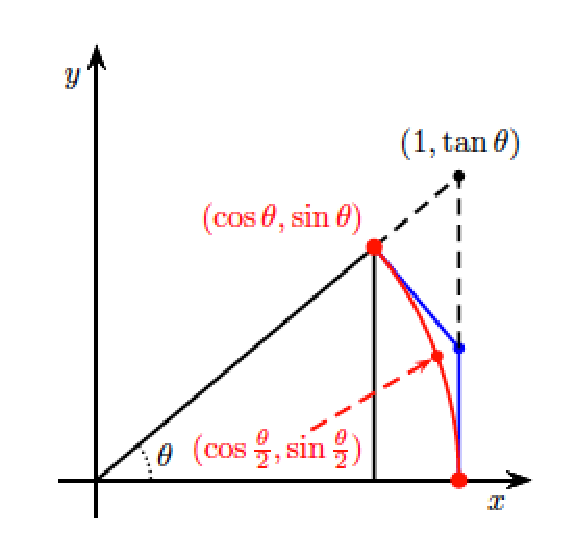
\includegraphics[clip, width=0.4\textwidth]{Graphics/SineTheta5-CS.eps}
\caption[A sample figure created as an \texttt{eps} file by \textsc{Matlab}]{PSTricks code for this figure is in the ``Graphics'' folder for the {\LaTeX} template.
The code was run using Xe{\LaTeX} and the resulting \texttt{pdf} file was converted to an \texttt{eps} file.}\label{FIGURE:fromPSTricks}
\end{center}
\end{figure}


\emph{Inkscape} is free and of high quality;
with this program, you should always keep the figures in Inkscape's native \textsc{svg} format,
and save them as \textsc{eps} only in order to view them in {\LaTeX}.


\begin{figure}[ht]
\label{fig2}
\begin{center}
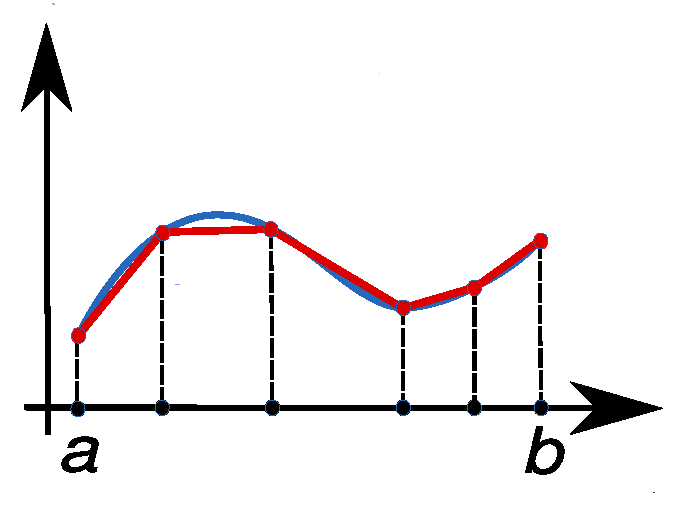
\includegraphics[width=0.4\textwidth]{Graphics/Figure1.eps}
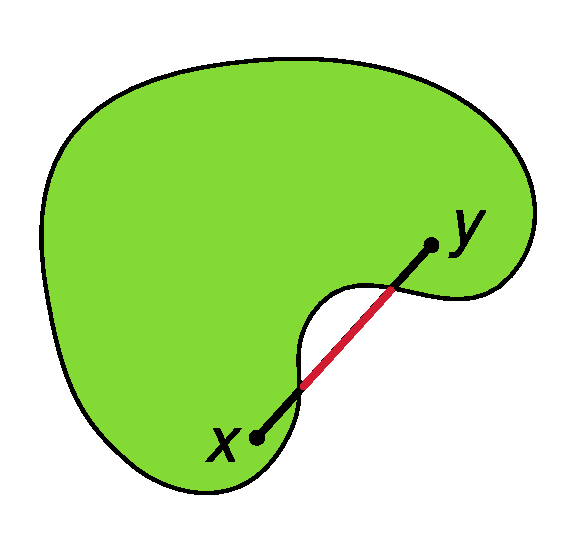
\includegraphics[width=0.309\textwidth]{Graphics/Figure2.eps}
\end{center}
\caption{A couple of figures drawn with Inkscape.}\label{FIGURE:fromInkScape}
\end{figure}

The two adjacent graphics in Figure \ref{FIGURE:fromInkScape} were created with Inkscape and exported to \textsc{eps}.
The figures in the original \textsc{svg} format are available in the report directory.
Note that the convention for punctuating a figure caption or table caption is pretty loose.
If an initial phrase is followed by a complete sentence, the phrase as well as any complete sentence should be ended with a period.
For consistency, it is \textsc{ok} to end all captions with a period even if a caption is just a phrase, as are all three captions illustrated here.

\section{Tables}

\noindent The next example is a simple table: Table \ref{TABLE:Simple}.
The {\LaTeX} code for it is presented after the table. 

% Note that the label follows the caption.
\begin{table}[h]
\begin{center}
  \begin{tabular}{|lcc|}
    \hline
    Date & High & Low\\ \hline
    1-Jul & 40 & 12\\
    2-Jul & 37 & 14\\
    3-Jul & 35 & 20\\ \hline
  \end{tabular}
\end{center}
\caption{A simple table showing fictional data.}\label{TABLE:Simple}
\end{table}

Look at the following source code for Table \ref{TABLE:Simple}, and note particularly how it is labeled.
The references to it in the two preceding sentencs were created by incorporating the label in the {\LaTeX} code 
(``\verb+Table \ref{TABLE:Simple}+'') used for creating this chapter.
Tables are labeled and referenced in a way similar to figures.

\begin{verbatim}
% Note that the label follows the caption.
\begin{table}[h]
\begin{center}
  \begin{tabular}{|lcc|}
    \hline
    Date & High & Low\\ \hline
    1-Jul & 40 & 12\\
    2-Jul & 37 & 14\\
    3-Jul & 35 & 20\\ \hline
  \end{tabular}
\end{center}
\caption{A sample table showing fictional data.}\label{TABLE:Simple}
\end{table}
\end{verbatim}

The next example, Table \ref{TABLE:SplitText}, illustrates a table in which column widths are specified by parameters in order to force long text to be spread over more than one line: 

\begin{table}[h]
\begin{center}
\begin{tabular}{|p{1in}|p{2in}|} \hline
Betty & Betty has a story to tell. \\ \hline
Bob   & Bob has a longer story to tell. \\ \hline
Bill  & Bill has a very much longer and far more dramatic story to tell. \\ \hline
\end{tabular}
\caption{A sample table with split lines of text.}\label{TABLE:SplitText}
\end{center}
\end{table}

\noindent Here's the code for Table \ref{TABLE:SplitText}:

\begin{verbatim}
\begin{table}[h]
\begin{center}
\begin{tabular}{|p{1in}|p{2in}|} \hline
Betty & Betty has a story to tell. \\ \hline
Bob   & Bob has a longer story to tell. \\ \hline
Bill  & Bill has a very much longer and far more dramatic story to tell. \\ \hline
\end{tabular}
\caption{A sample table with split lines of text.}\label{TABLE:SplitText}
\end{center}
\end{table}
\end{verbatim}

\subsubsection{Style tips about figures and tables}
You should always make sure that your figures are easy to see, so for example, make sure that any curves are not too thin or text is not too small.
And don't forget to include axis labels with units specified.

Your figures should look good both in color and as black-and-white, since for presentations you will most likely want figures in color, while in a printed report all the figures will usually be printed in black-and-white (and then, what looks very clear and pretty on your screen may appear as a dark region on paper).

Good captions greatly improve the usefulness of figures and tables.

But no matter how well a caption describes a figure or table, you should always reference it and explain it in your text.
You may feel you are being redundant, but your readers won't think so:
a picture with a good description is worth a thousand words, and a picture without a description in the text is left dangling.

\section{Picking nits}
Notice that in this sample report, all of the captions for figures and tables are placed below the object, and their labels end with a numbered identifier---e.g., Figure 4.1, Table 4.2---terminated with a colon (``:'') inserted automatically by the {\LaTeX} compiler. 
\emph{The Chicago Manual of Style} specifies the use of a period (``.'') to follow the figure number and a blank space to follow the table number, and \emph{New Hart's Rules} follows both figure and table numbers with a blank space.  
Moreover, \emph{New Hart's Rules} places table captions above the table, rather than beneath.
But here we bow to usage in {Gr\"{a}tzer's} \emph{More Math Into {\LaTeX}}(See Bibliography for references).
In such minutiae it's your choice, but remember, consistency (perhaps a hobgoblin of lesser minds but certainly a ruling passion in typography) is standard practice. 


Another place to be on guard is in referencing, e.g., sections, equations, and lemmas.
Do you capitalize or leave it in lower case: Chapter 1 or chapter 1, Theorem 1 or theorem 1, Lemma 1 or lemma 1?
Of course at sentence heads you have no choice but to capitalize.
When you refer to a figure or a table, you may write, for example, ``Fig. 1'', ``Figure 1'', with or without an initial capital, and write ``Table 1'' or ``table 1''.
Recommended usage for this report is to use proper nouns: whether abreviated or spelled out in full, capitalize the labels.
It's up to you, but be consistent.

You'll think of other things as you go along.
Just consider how it looks on the page, and {\it be consistent throughout your report}.

\endinput



% Chapter 5
\ifthenelse{\boolean{@twoside}}{\myclearpage}{}
\chapter{Results and Discussion}
\label{Ch:Result and Discussion}
\section{Q-Learning}

\subsection{Basic Model}
To build basic model, we used portfolio value change as a reward function, which means the agent will choose the action that will increase the expected portfolio value the most. We used two decimal of price change pair as a state.

We adjusted the parameters to give better performance. The learning rate($\alpha$), which decides the impact of new data on the existing Q-table, was set as 0.0001 based on experiment. The discount factor($\gamma$), which discounts the sum of future reward was set as 0.9. The epsilon($\epsilon$) was set as 0.9 and for every time period it is decreased 1\% until it reaches 0.01. It is in order to let the actions be chosen more randomly for exploration in the earlier times, since Q-table doesn’t contain much information. However later times’ actions are more likely to be chosen based on Q-table with smaller epsilon value. With those parameters, we trained the Q-table for each dataset 3000 episodes each.

As we trained on 10 training datasets, the performances of the basic model on each dataset didn’t have distinct patterns. Usually, the portfolio gains by the model were way better(3~4 times final portfolio value) than benchmark, but training results from 4th, 7th, 8th, 9th training set were similar or even below the benchmark gains. Each plot below has two subplots. The upper plot shows how the final portfolio value changes over every episode, and using the last episode’s data we drew bottom plot which shows the portfolio value change over days. Compared to those of training 1 with KLAC and SKX data and training 10 with NVDA and SKX data, the results of training 4 and training 9 are not good. We didn’t find any clear reason behind this. The dimension of Q-table is steadily increased with more training as shown in below plot.

\begin{figure}[H]
\begin{subfigure}{.5\textwidth}%
\centering
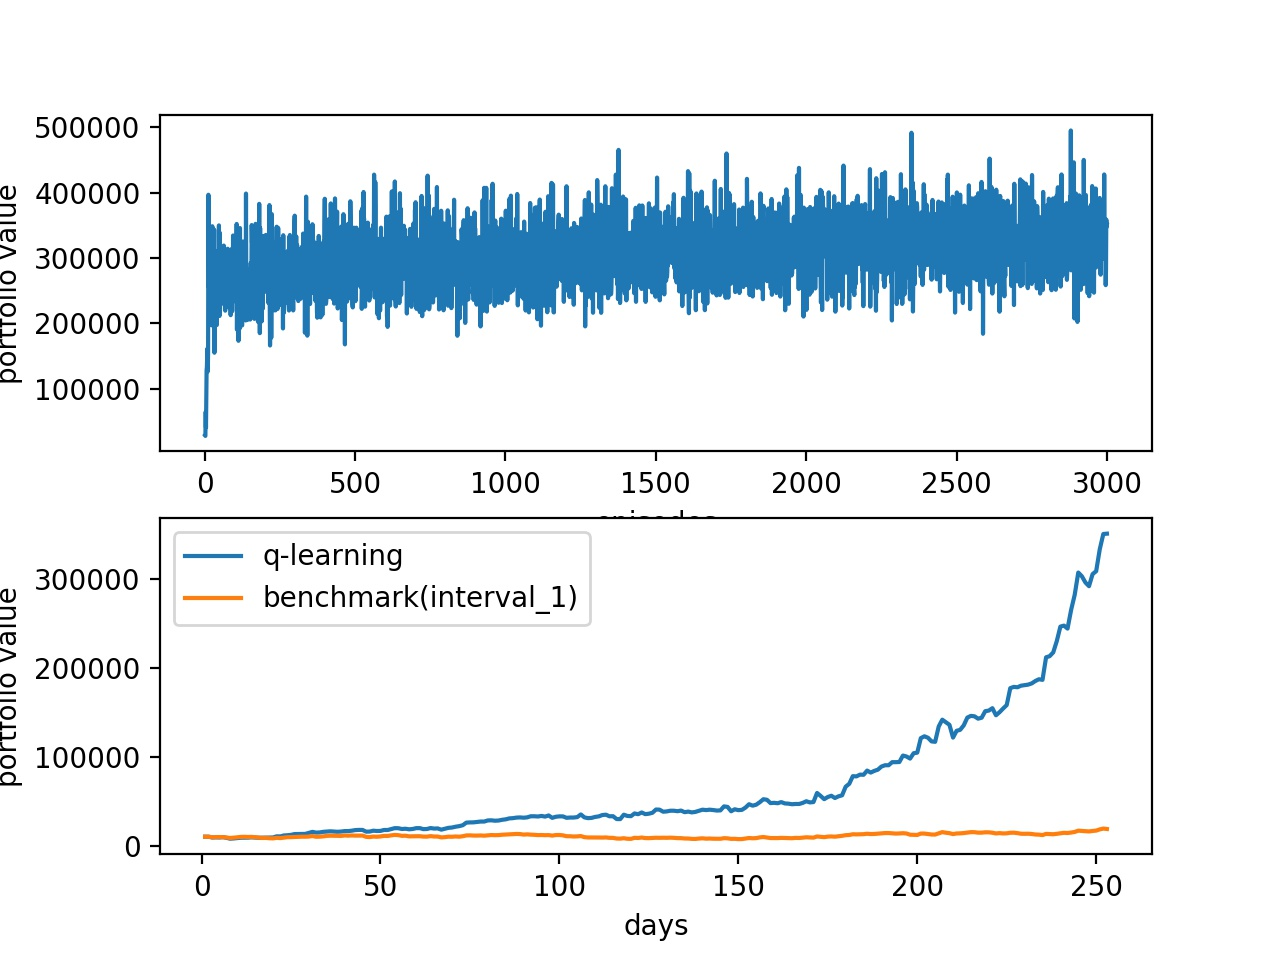
\includegraphics[clip, width=1.1\textwidth]{Graphics/q_learning_KS1.eps} \caption{Training 1 (KLAC \& SKX)} 
\end{subfigure}%
\begin{subfigure}{.5\textwidth}%
\centering
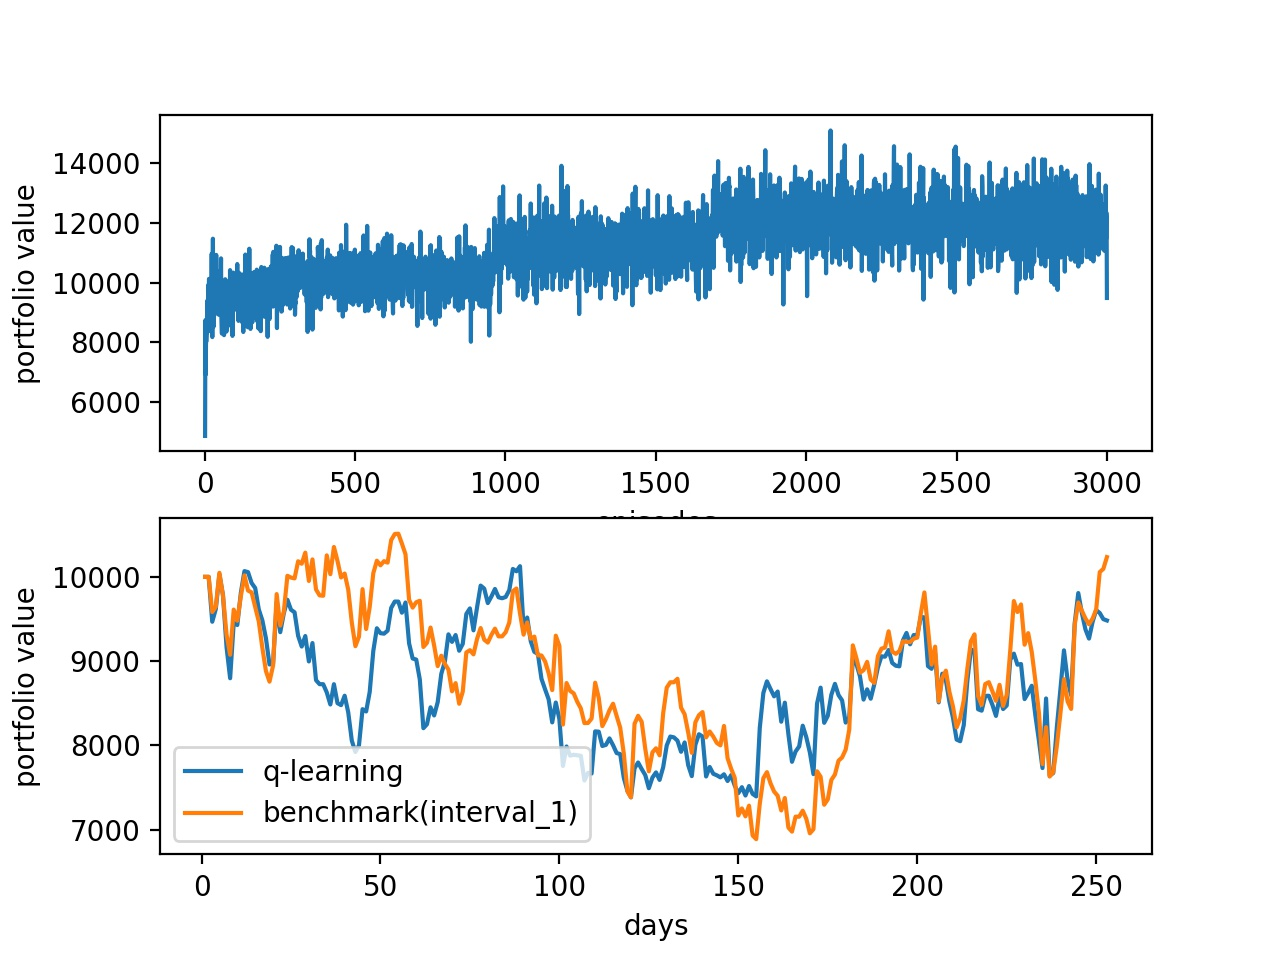
\includegraphics[clip, width=1.1\textwidth]{Graphics/q_learning_AM4.jpg} \caption{Training 4 (AMD \& MTN)}
\end{subfigure}%
\vspace{0.1cm}
\begin{subfigure}{.5\textwidth}%
\centering
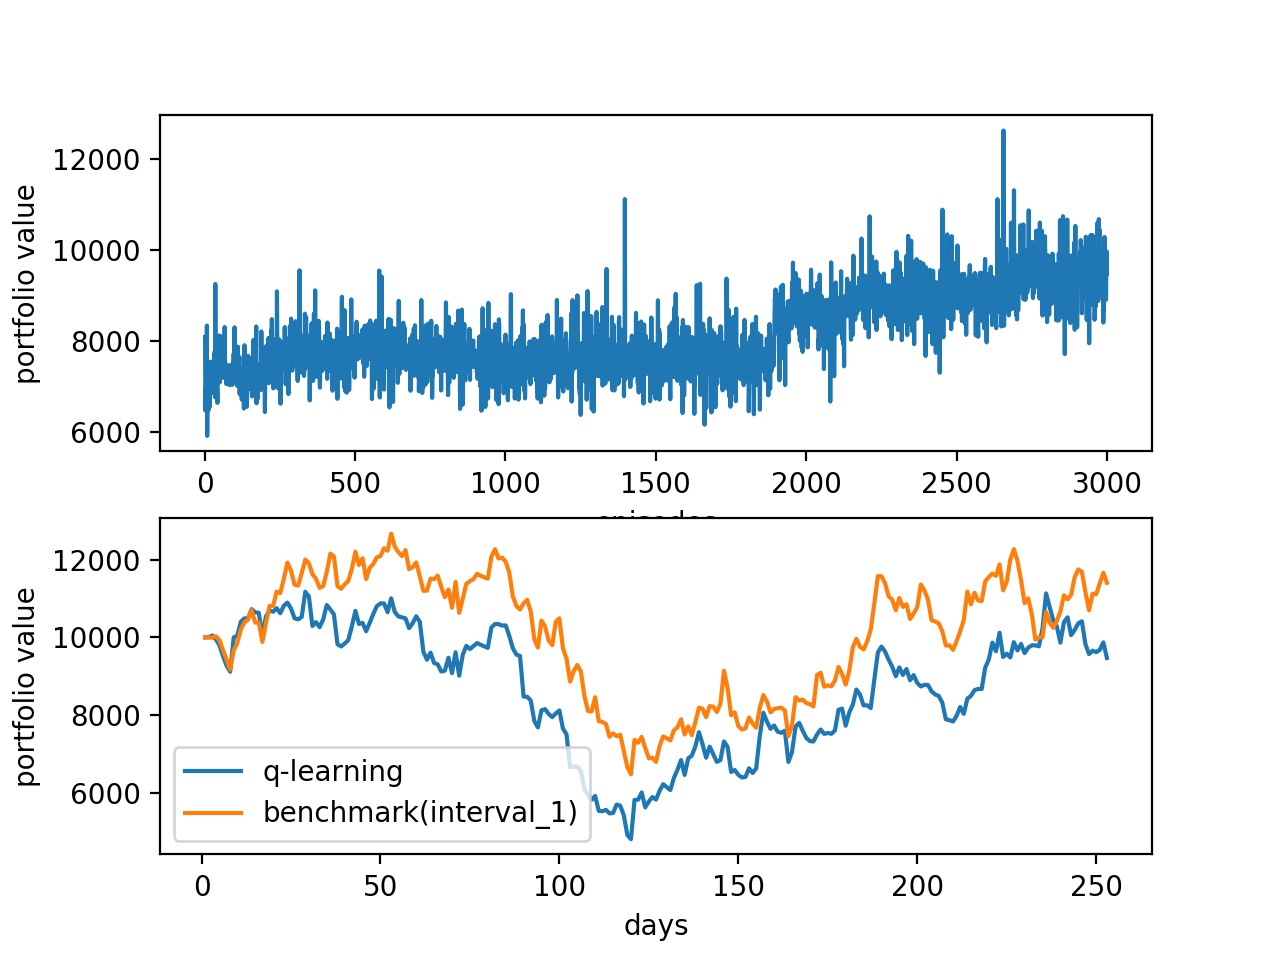
\includegraphics[clip, width=1.1\textwidth]{Graphics/q_learning_MP9.jpg} \caption{Training 9 (MU \& PPC)}
\end{subfigure}%
\begin{subfigure}{.5\textwidth}
\centering
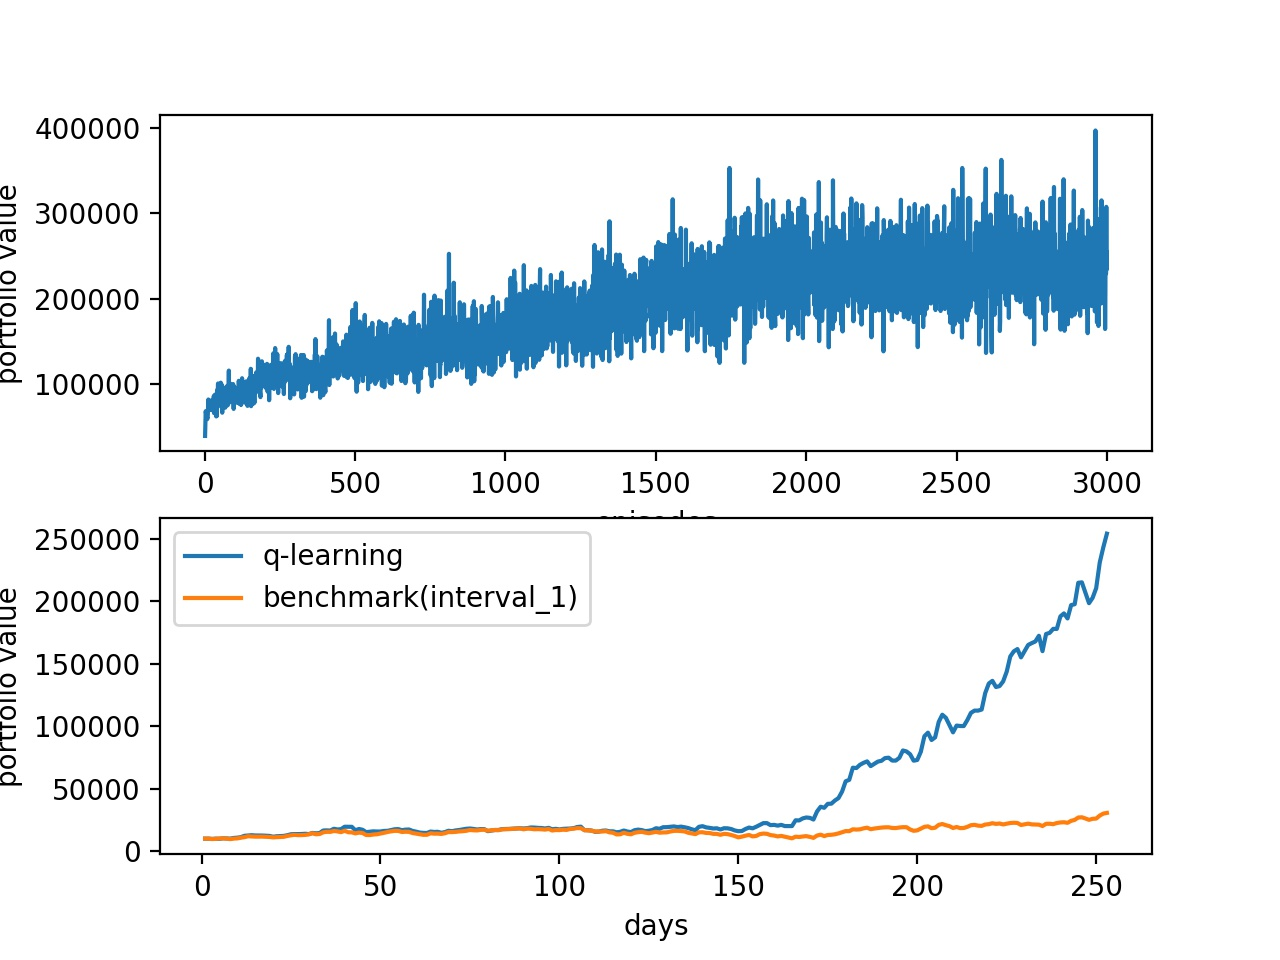
\includegraphics[clip, width=1.1\textwidth]{Graphics/q_learning_NS10.jpg} \caption{Training 10 (NVDA \& SKX)}
\end{subfigure}%
\vspace{0.1cm}
\begin{figure}
\begin{center}
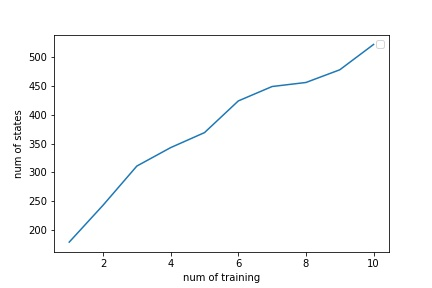
\includegraphics[clip, width=0.8\textwidth]{Graphics/dimension.jpg} \caption{Dimension change over training}
\end{center}
\end{figure}
\end{figure}%

Using the $Q$-table we trained, we tested on two test datasets(AMAT \& CAJ, FCX \& CAJ). Test results using FCX \& CAJ dataset usually showed better results. However more training didn’t guarantee better test results. For AMAT \& CAJ, the best test result was using the Q-table trained with 1 dataset, and further training tables made the test results’ portfolio value be decreased. On the other hand, for FCX \& CAJ, the best test result was with 8 times training Q-table, and before and after that the final portfolio value is below benchmarks. To check the reason why test results keep changing, we analyzed the actions taken in each result. Even the actions taken in the test using 9 times training, and using 10 times training differed a lot. The last plot which has 3 subplots is drawn using the FCX \& CAJ data. The first subplot is comparing the actions taken with 5 and 8 times training, while the second is comparing 8 times and 10 times, and the last is comparing 10 times and 9 times.
\vspace{0.05cm}
\begin{figure}[H]
\begin{figure}[H]
\begin{center}
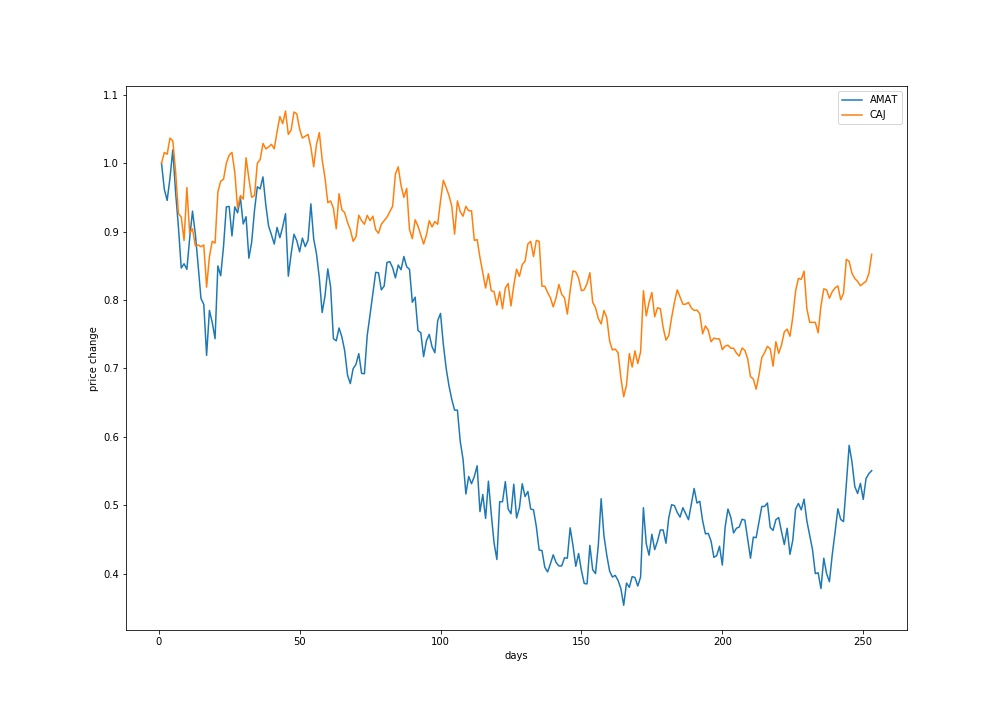
\includegraphics[clip, width=0.7\textwidth]{Graphics/test1_pricechange.jpg} \caption{TEST SET1 (AMAT \& CAJ) :PRICE CHANGE}
\end{center}
\end{figure}
\vspace{0.1cm}
\begin{subfigure}{.5\textwidth}%
\centering
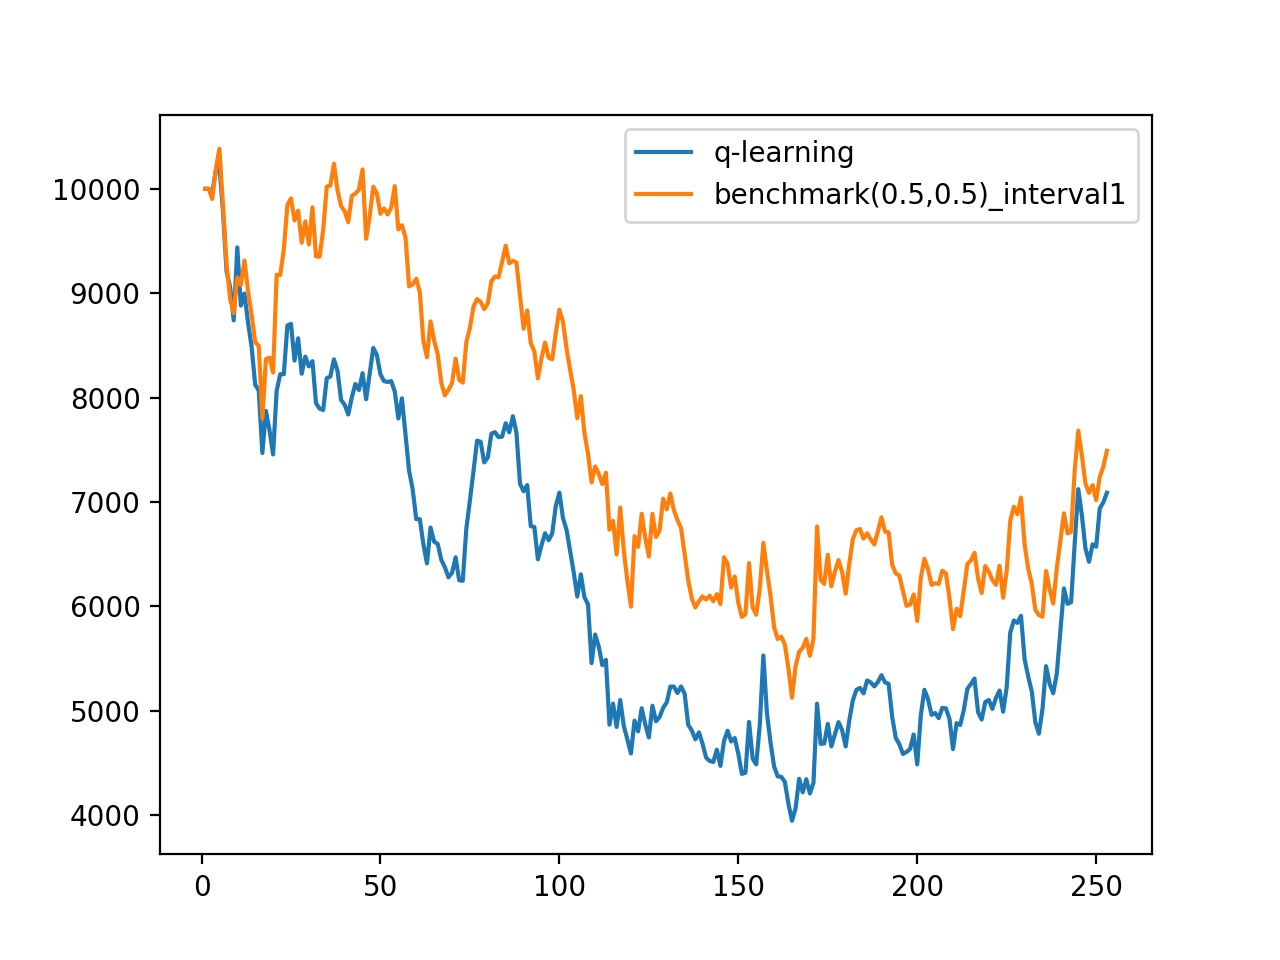
\includegraphics[clip, width=1.1\textwidth]{Graphics/test_KS1_AC_action.jpg} \caption{TEST SET1 (AMAT \& CAJ):1 training} 
\end{subfigure}%
\vspace{0.1cm}
\begin{subfigure}{.5\textwidth}%
\centering
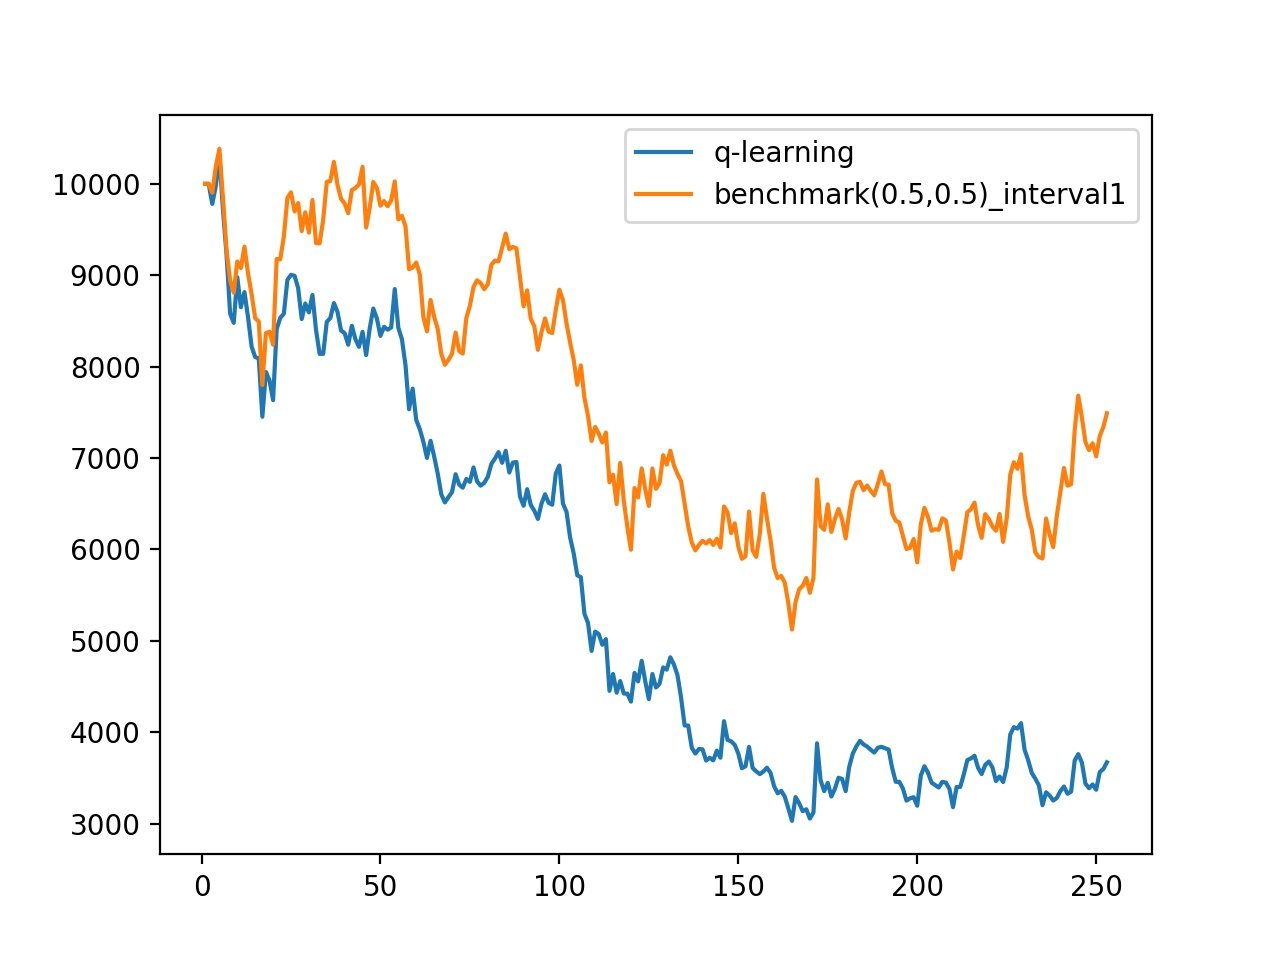
\includegraphics[clip, width=1.1\textwidth]{Graphics/test_LP3_AC_action.jpg} \caption{TEST SET1 (AMAT \& CAJ):3 training}
\end{subfigure}%
\end{figure}%

\newpage

\begin{figure}[H]
\begin{figure}[H]
\begin{center}
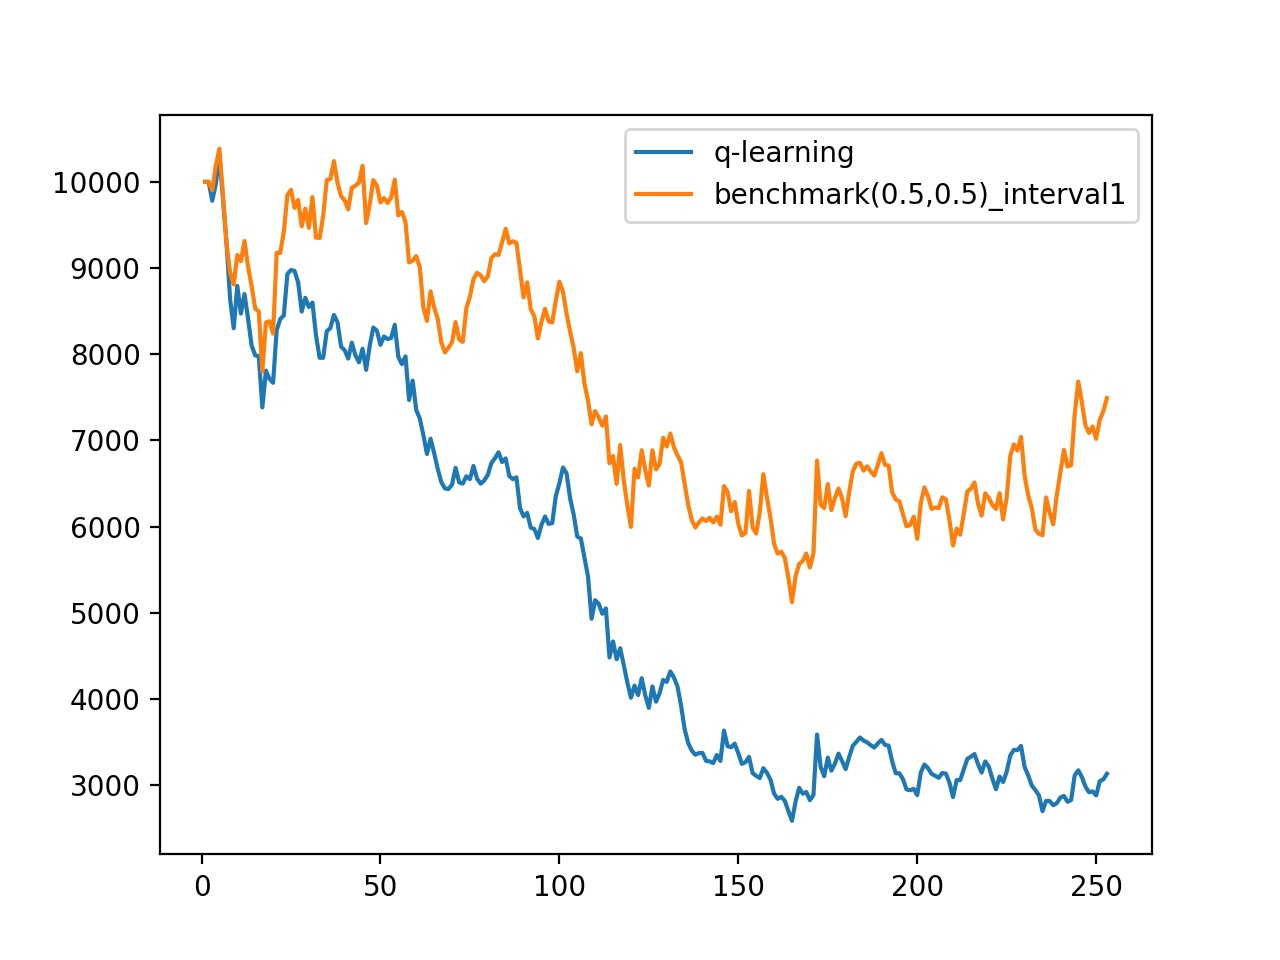
\includegraphics[clip, width=0.9\textwidth]{Graphics/test_NS10_AC_action.jpg} \caption{TEST SET1 (AMAT \& CAJ) : result with 10 training Q-table}
\end{center}
\end{figure}
\vspace{0.1cm}
\begin{figure}[H]
\begin{center}
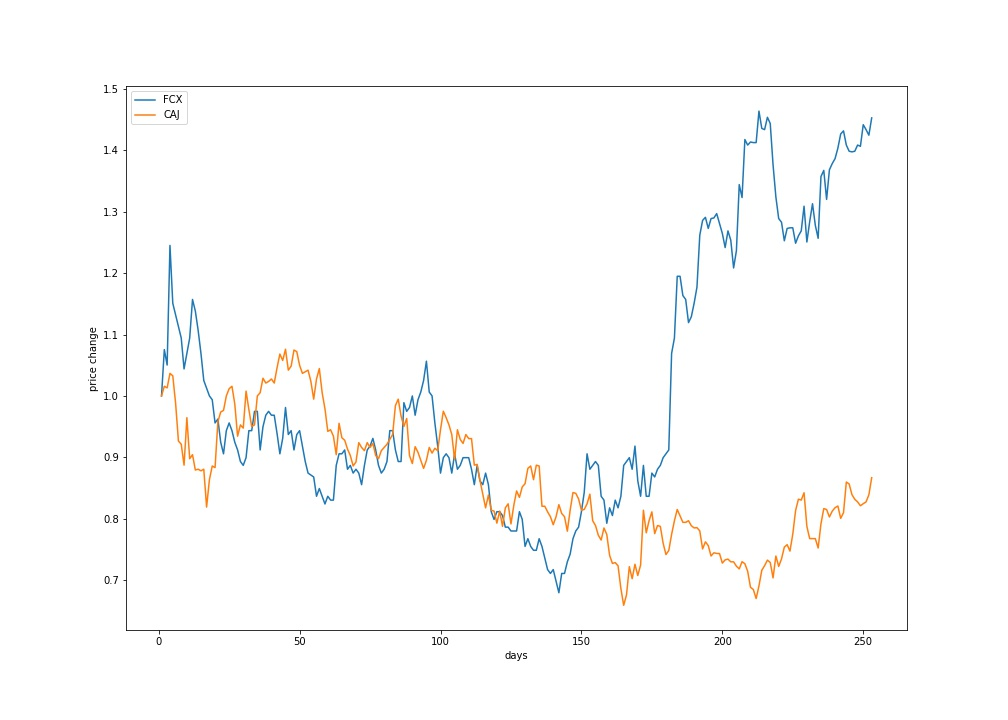
\includegraphics[clip, width=0.9\textwidth]{Graphics/test2_pricechange.jpg} \caption{TEST SET2 (FCX \& CAJ) : PRICE CHANGE}
\end{center}
\end{figure}
\vspace{0.1cm}
\end{figure}

\newpage

\begin{figure}[H]
\begin{subfigure}{.5\textwidth}%
\centering
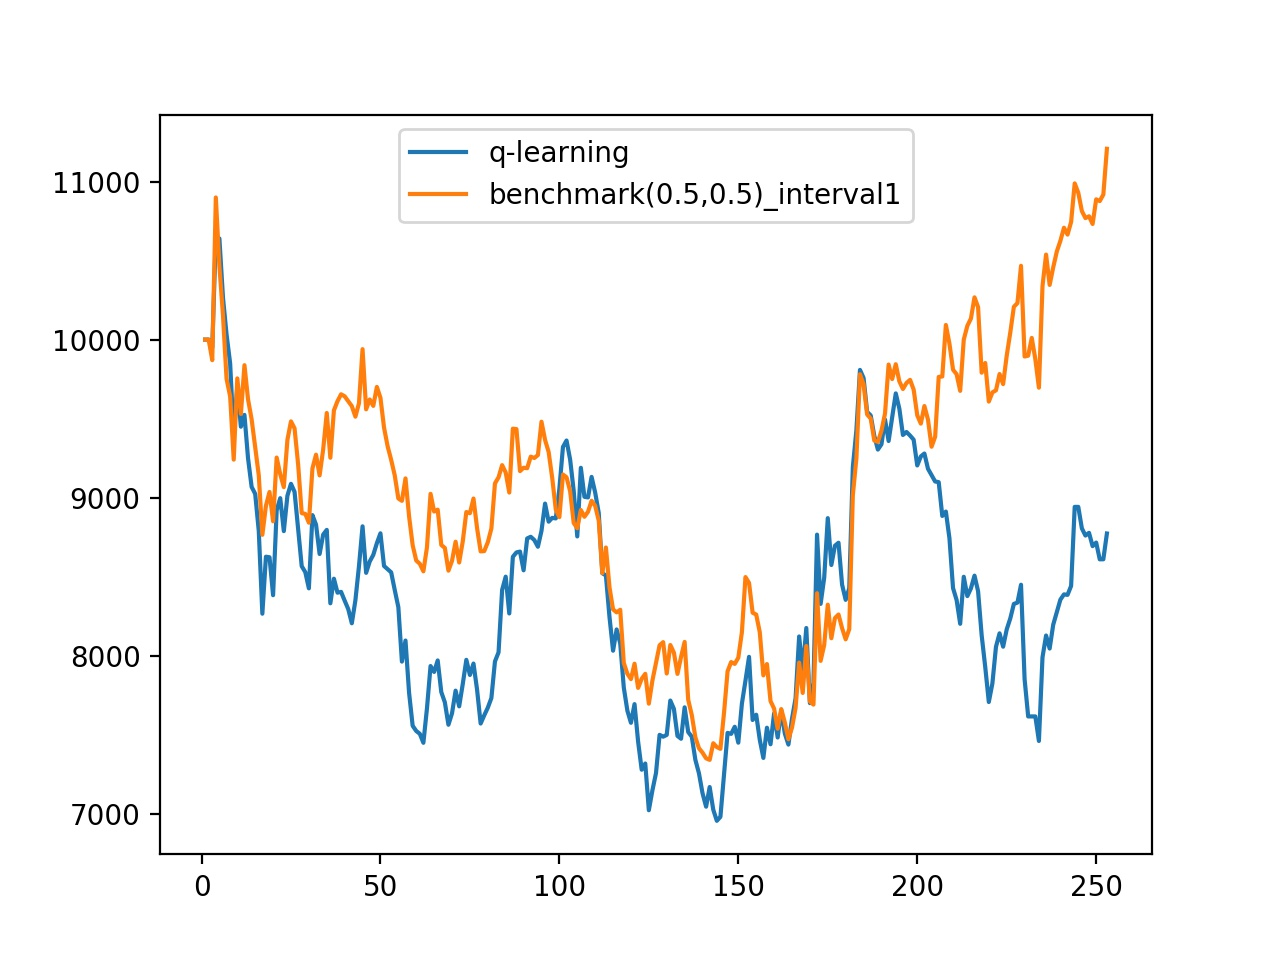
\includegraphics[clip, width=0.9\textwidth]{Graphics/test_NM5_FC_action.jpg} \caption{TEST SET2 (FCX \& CAJ): 5 training} 
\end{subfigure}%
\vspace{0.1cm}
\begin{subfigure}{.5\textwidth}%
\centering
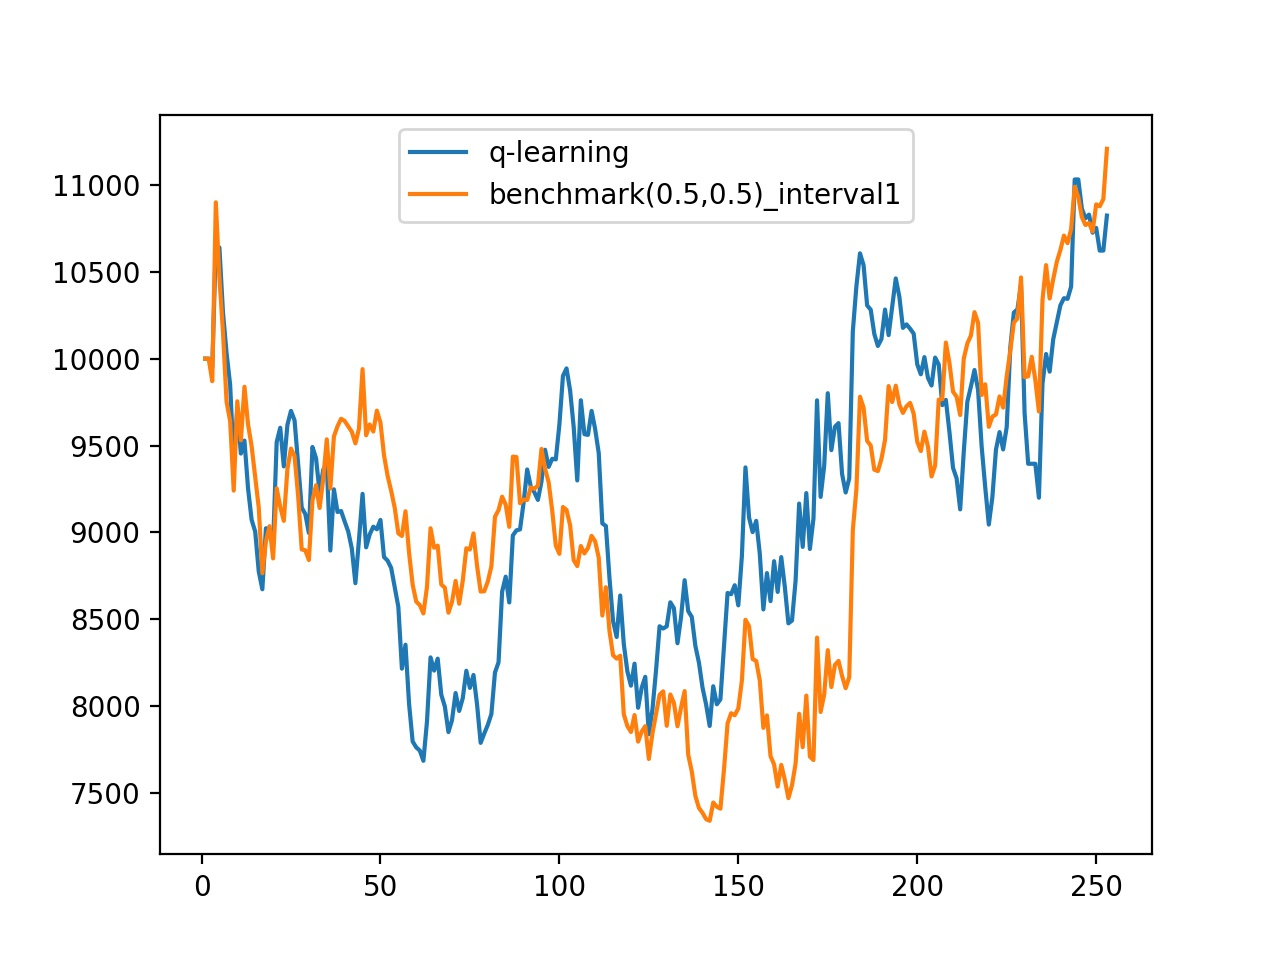
\includegraphics[clip, width=0.9\textwidth]{Graphics/test_AS8_FC_action.jpg} \caption{TEST SET2 (FCX \& CAJ): 8 training}
\end{subfigure}%
\begin{figure}[H]
\begin{center}
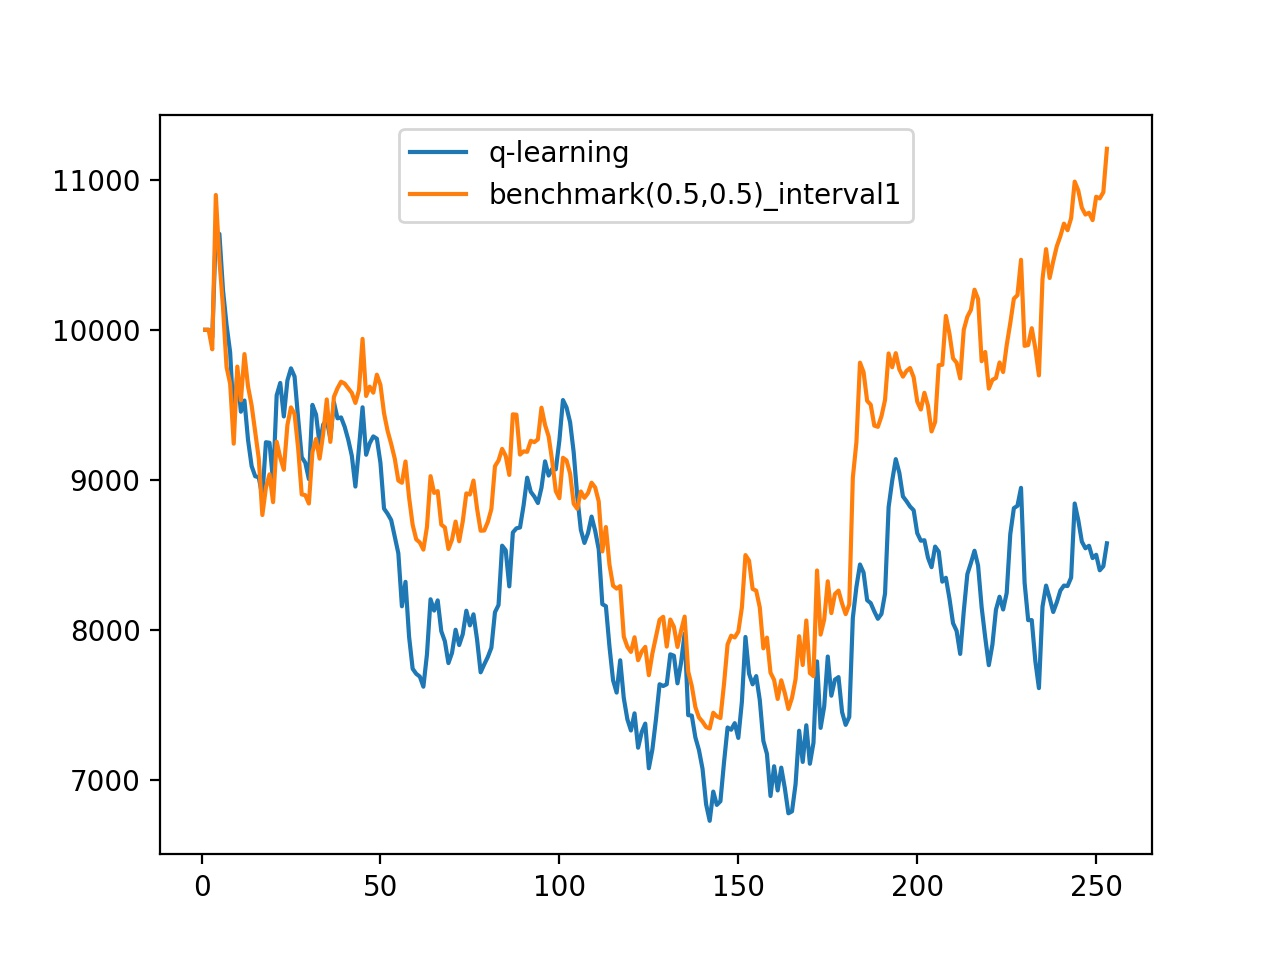
\includegraphics[clip, width=0.6\textwidth]{Graphics/test_NS10_FC_action.jpg} \caption{TEST SET2 (FCX \& CAJ) : result with 10 training Q-table}
\end{center}
\end{figure}
\begin{figure}[H]
\begin{center}
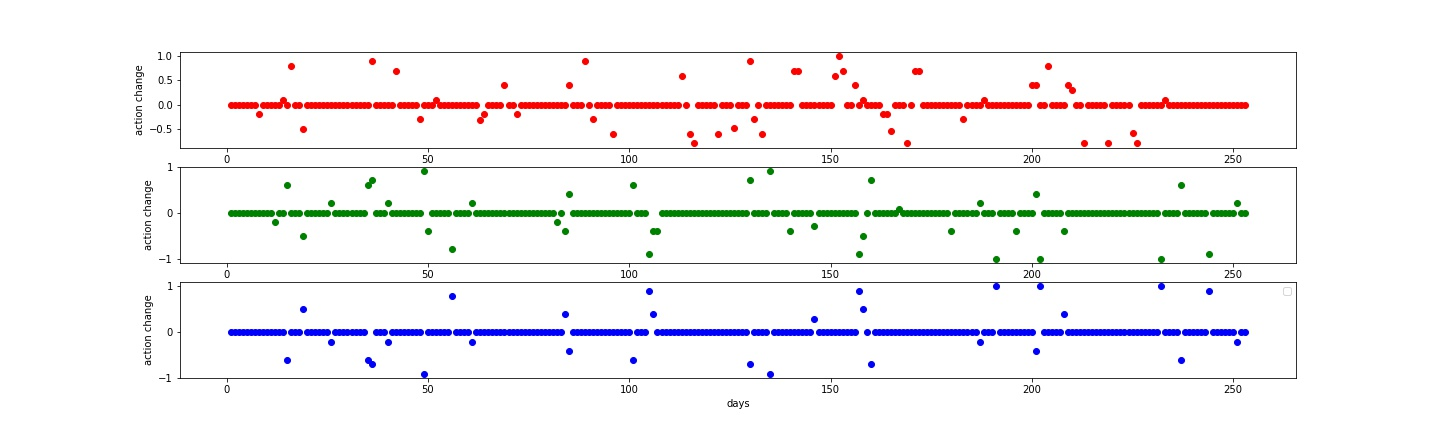
\includegraphics[clip, width=0.7\textwidth]{Graphics/actionchange3.jpg} \caption{ACTION CHANGE : (8 vs 5, 8 vs 10, 10 vs 9)}
\end{center}
\end{figure}
\end{figure}

\subsection{Linear Regression}
As for portfolio management, we should not only consider the  profit, but also the risk, thus we use the sharpe ratio $R=\frac{E(Rp)-Rf}{\sigma Rp}$ as reward function, where $E(Rp)$ is the expected portfolio return , $Rf$ is the risk free rate, and $\sigma Rp$ is the portfolio standard deviation. In our model, we let $Rf=0$, and $Rf=\frac{pv_t-pv_{t-1}}{pv_{t-1}}$. We use the pairs of two stocks’ simple linear regression functions’ slope as states $(a_n,k_n)$, and to generalize the states, we only keep one decimal of the slope.

\vspace{0.5cm}

\textbf{Using 10 pairs’s stocks’ one year data to train the} model
\begin{figure}[H]
\begin{subfigure}{.5\textwidth}%
\centering
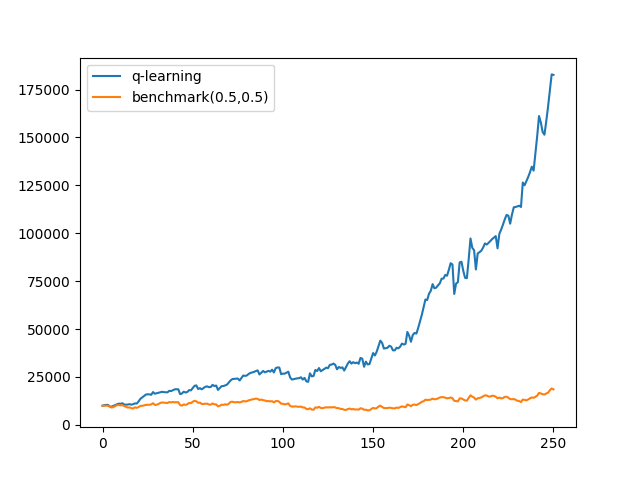
\includegraphics[clip, width=0.9\textwidth]{Graphics/trainParameterWithT.png} \caption{TRAIN 1 (KLAC \& SKX)
} 
\end{subfigure}%
\begin{subfigure}{.5\textwidth}%
\centering
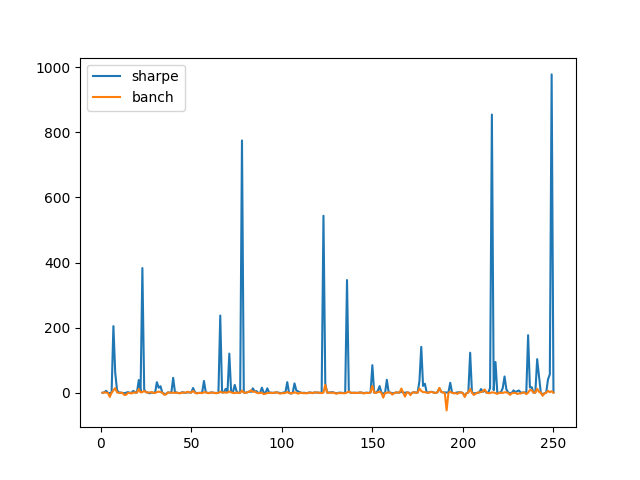
\includegraphics[clip, width=0.9\textwidth]{Graphics/trainParameterWTSharpe.png} \caption{Sharpe Ratio of TRAIN 1}
\end{subfigure}%
\vspace{0.1cm}
\begin{subfigure}{.5\textwidth}%
\centering
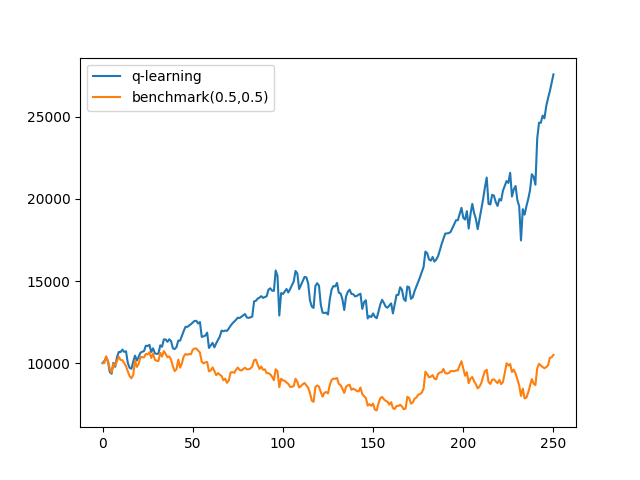
\includegraphics[clip, width=0.9\textwidth]{Graphics/trainParameter3WT.png} \caption{TRAIN 4 (AMD \& MTN))} 
\end{subfigure}%
\begin{subfigure}{.5\textwidth}%
\centering
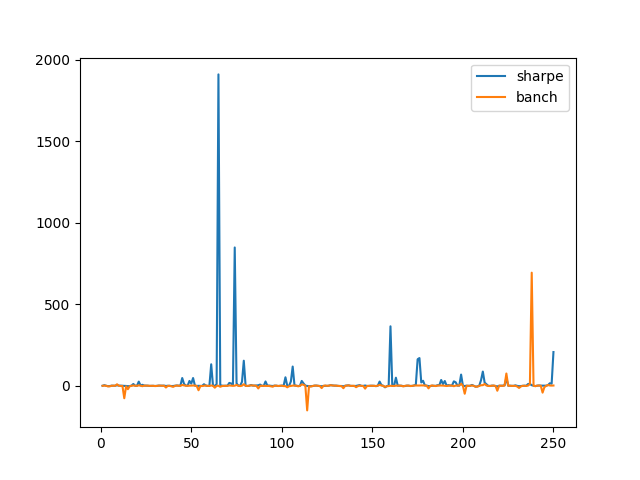
\includegraphics[clip, width=0.9\textwidth]{Graphics/trainParameter3WTS.png} \caption{Sharpe Ratio of TRAIN 4}
\end{subfigure}%
\vspace{0.1cm}
\begin{subfigure}{.5\textwidth}%
\centering
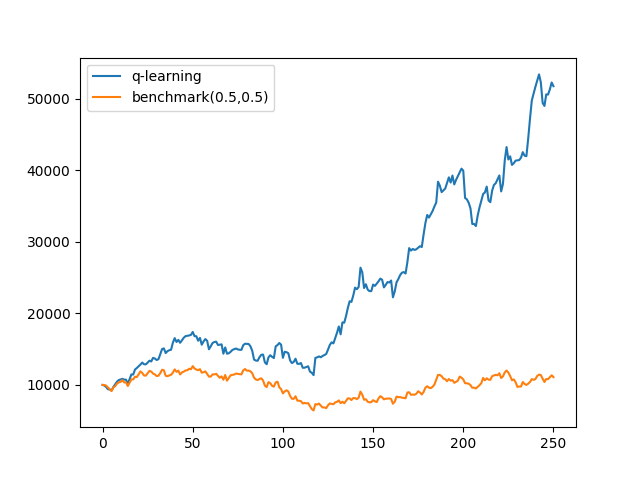
\includegraphics[clip, width=0.9\textwidth]{Graphics/trainPA9.png} \caption{TRAIN 9 (MU \& PPC))} 
\end{subfigure}%
\begin{subfigure}{.5\textwidth}%
\centering
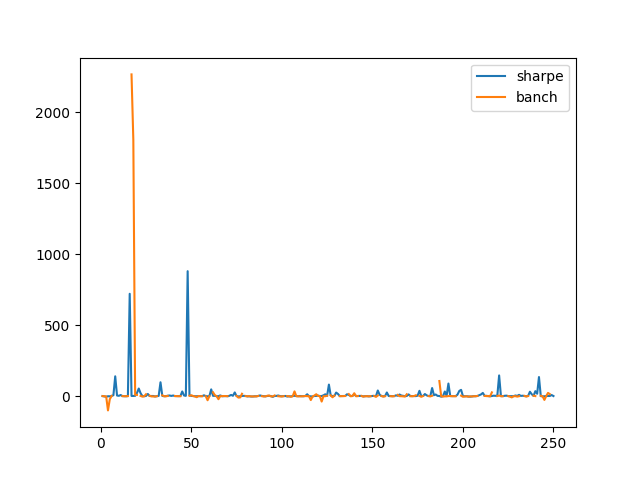
\includegraphics[clip, width=0.9\textwidth]{Graphics/trainPA9S.png} \caption{Sharpe Ratio of TRAIN 9}
\end{subfigure}%
\end{figure}

\newpage
Then we get the test result as follow:

\begin{figure}[H]
\begin{subfigure}{.5\textwidth}%
\centering
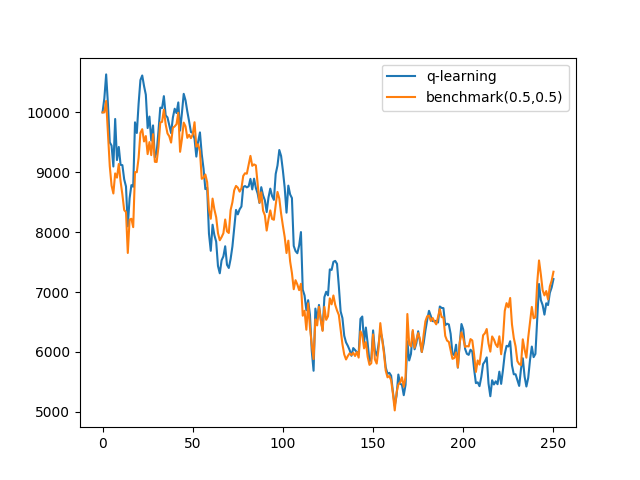
\includegraphics[clip, width=0.9\textwidth]{Graphics/TestAC3.png} \caption{TEST 1 (AMAT \& CAJ)} 
\end{subfigure}%
\begin{subfigure}{.5\textwidth}%
\centering
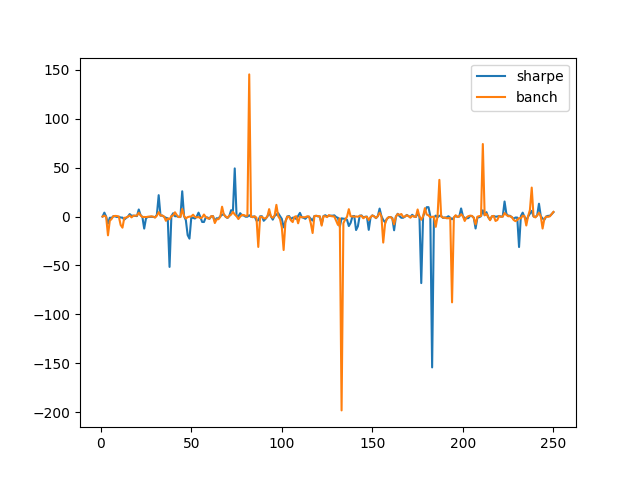
\includegraphics[clip, width=0.9\textwidth]{Graphics/TESTAC3S.png} \caption{Sharpe Ratio of TEST 1}
\end{subfigure}%
\vspace{0.1cm}
\begin{subfigure}{.5\textwidth}%
\centering
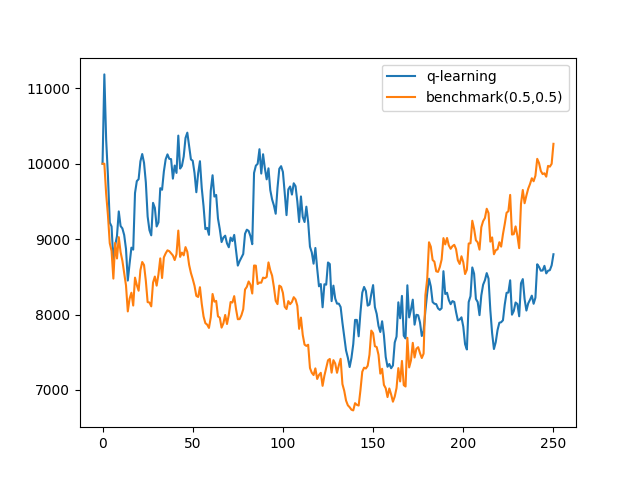
\includegraphics[clip, width=0.9\textwidth]{Graphics/TESTFC3.png} \caption{TEST 2 (FCX \& CAJ))} 
\end{subfigure}%
\begin{subfigure}{.5\textwidth}%
\centering
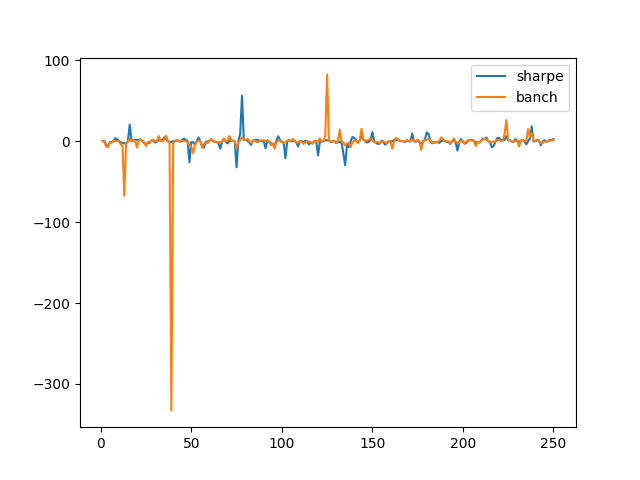
\includegraphics[clip, width=0.9\textwidth]{Graphics/TESTFC3S.png} \caption{Sharpe Ratio of TEST 2}
\end{subfigure}%
\vspace{0.7cm}
We are thinking that whether more days of a period can have a better result, so we use each 10 days as a period to get the regression functions.
\vspace{0.7cm}
\begin{subfigure}{.5\textwidth}%
\centering
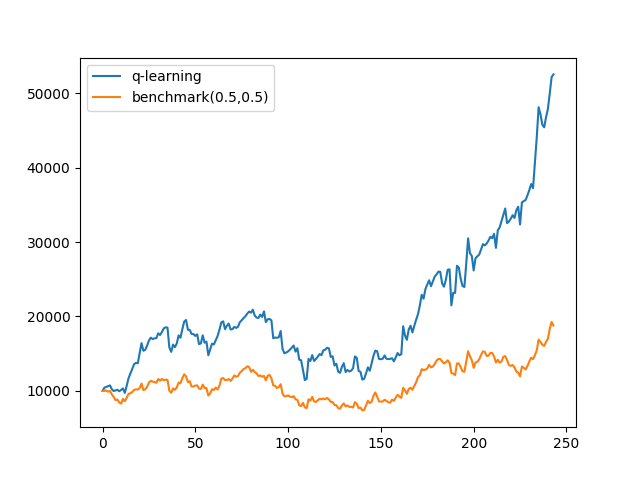
\includegraphics[clip, width=0.9\textwidth]{Graphics/trainPA00WT.png} \caption{TRAIN 1 (KLAC \& SKX)} 
\end{subfigure}%
\begin{subfigure}{.5\textwidth}%
\centering
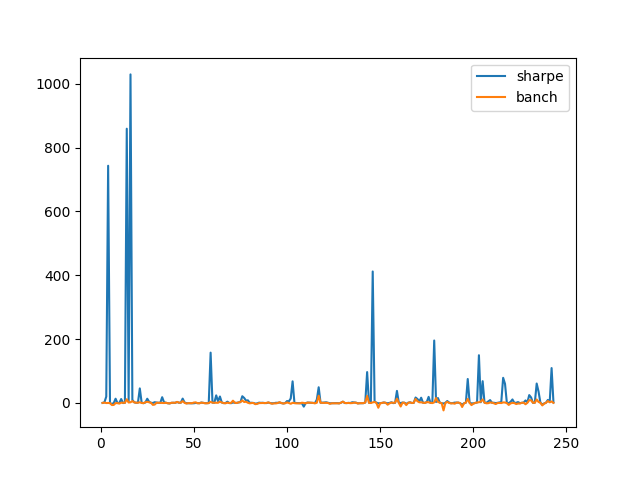
\includegraphics[clip, width=0.9\textwidth]{Graphics/trainPA00S.png} \caption{Sharpe Ratio of TRAIN 1}
\end{subfigure}%
\end{figure}

\newpage
\begin{figure}[H]
\begin{subfigure}{.5\textwidth}%
\centering
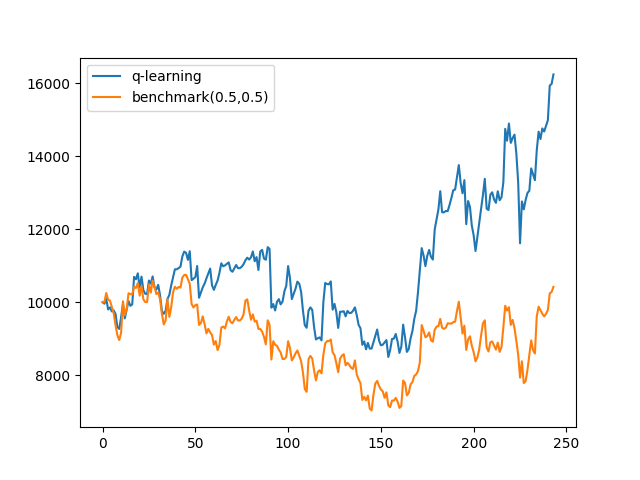
\includegraphics[clip, width=0.9\textwidth]{Graphics/trainPA33.png} \caption{TRAIN 4 (AMD \& MTN))} 
\end{subfigure}%
\begin{subfigure}{.5\textwidth}%
\centering
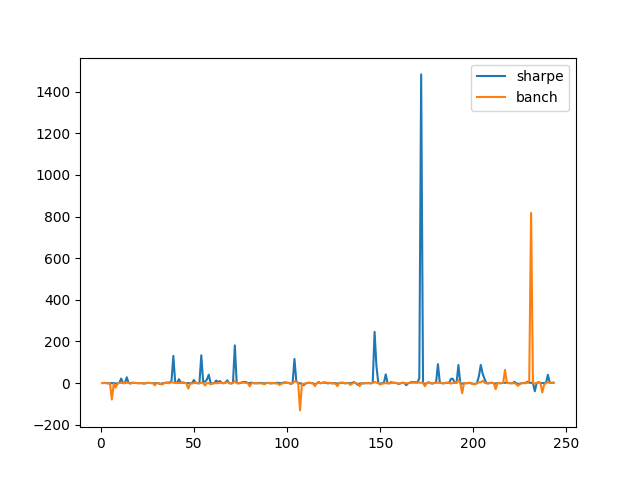
\includegraphics[clip, width=0.9\textwidth]{Graphics/trainPA33S.png} \caption{Sharpe Ratio of TRAIN 4}
\end{subfigure}%
\vspace{0.1cm}
\begin{subfigure}{.5\textwidth}%
\centering
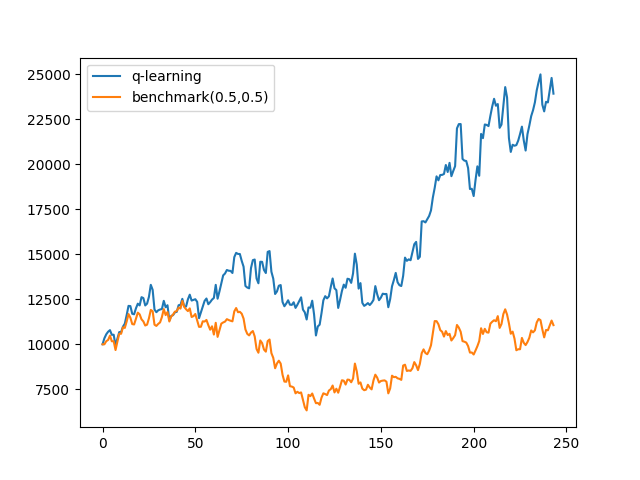
\includegraphics[clip, width=0.9\textwidth]{Graphics/trainPA99.png} \caption{TRAIN 9 (MU \& PPC))} 
\end{subfigure}%
\begin{subfigure}{.5\textwidth}%
\centering
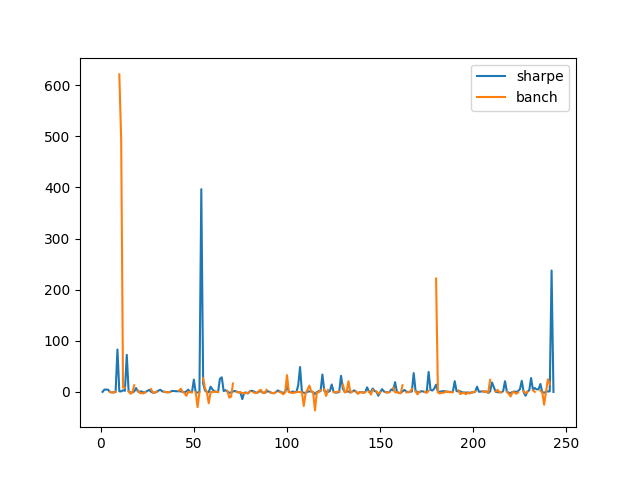
\includegraphics[clip, width=0.9\textwidth]{Graphics/trainPA99s.png} \caption{Sharpe Ratio of TRAIN 9}
\end{subfigure}%
\vspace{0.7cm}

Then we get the test result as follow:

\vspace{0.4cm}
\begin{subfigure}{.5\textwidth}%
\centering
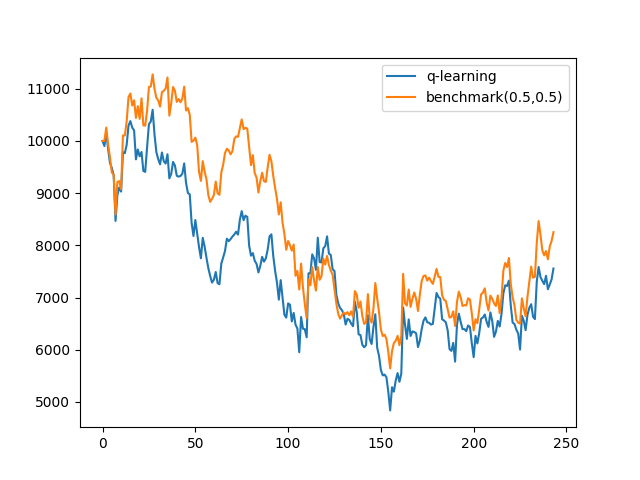
\includegraphics[clip, width=0.9\textwidth]{Graphics/TESTAC10.png} \caption{TEST 1 (AMAT \& CAJ)} 
\end{subfigure}%
\begin{subfigure}{.5\textwidth}%
\centering
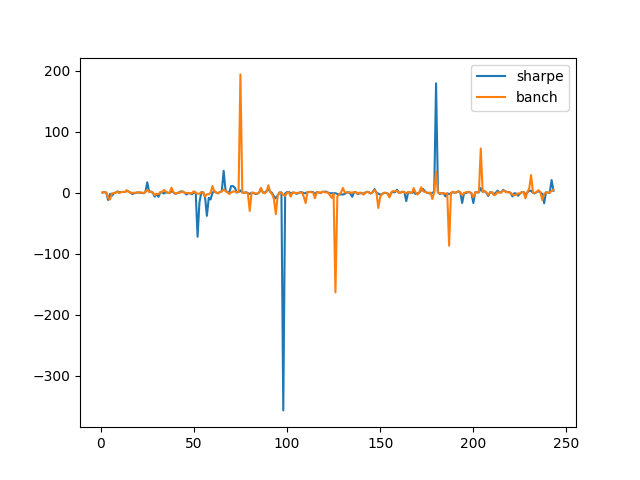
\includegraphics[clip, width=0.9\textwidth]{Graphics/TESTAC10S.png} \caption{Sharpe Ratio of TEST 1}
\end{subfigure}%
\end{figure}

\newpage
\begin{figure}[H]
\begin{subfigure}{.5\textwidth}%
\centering
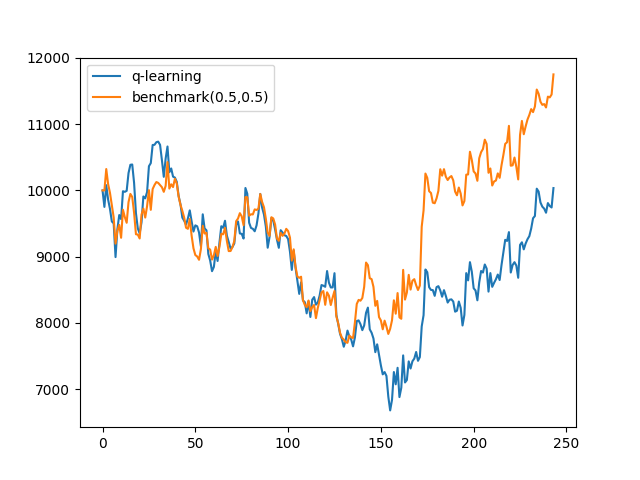
\includegraphics[clip, width=0.9\textwidth]{Graphics/TESTFC10.png} \caption{TEST 2 (FCX \& CAJ)} 
\end{subfigure}%
\begin{subfigure}{.5\textwidth}%
\centering
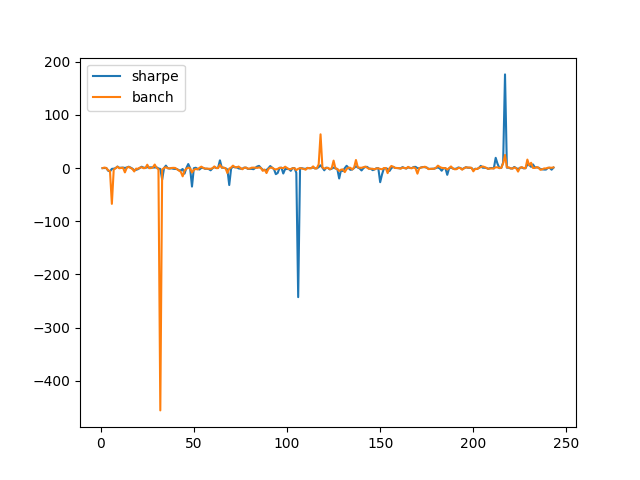
\includegraphics[clip, width=0.9\textwidth]{Graphics/TESTFC10S.png} \caption{Sharpe Ratio of TEST 2}
\end{subfigure}%
\vspace{0.4cm}

It is even worse than we use 3 days as a period.

\vspace{0.4cm}

However, if we use 3 days’ regression to test in the 10-day training q-table, we get the following testing result:

\vspace{0.4cm}

\begin{subfigure}{.5\textwidth}%
\centering
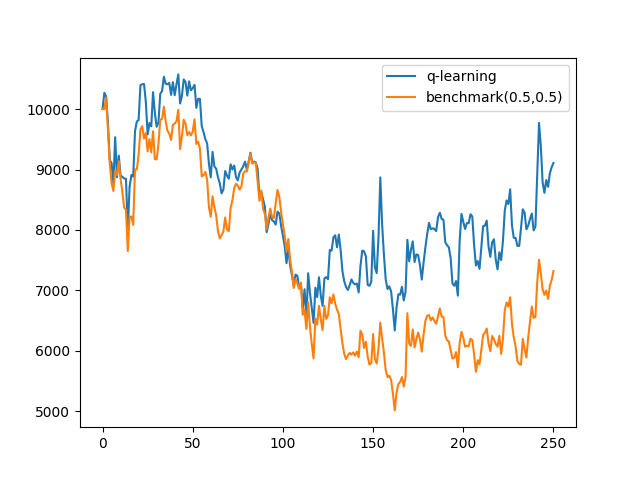
\includegraphics[clip, width=0.9\textwidth]{Graphics/TESTAC3Dby10train.png} \caption{TEST 1 (AMAT \& CAJ)} 
\end{subfigure}%
\begin{subfigure}{.5\textwidth}%
\centering
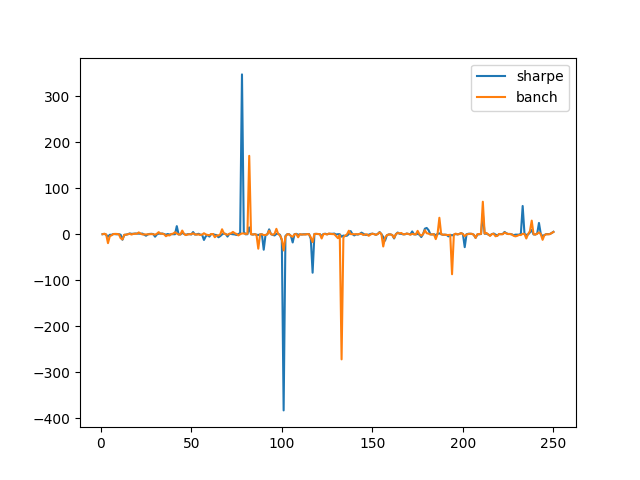
\includegraphics[clip, width=0.9\textwidth]{Graphics/TESTAC3Dby10trainS.png} \caption{Sharpe Ratio of TEST 1}
\end{subfigure}%
\vspace{0.4cm}
\begin{subfigure}{.5\textwidth}%
\centering
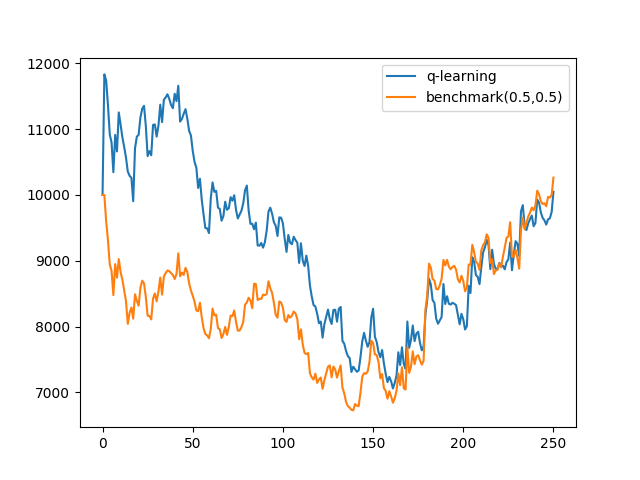
\includegraphics[clip, width=0.9\textwidth]{Graphics/TESTFC3Dby10train.png} \caption{TEST 1 (AMAT \& CAJ)} 
\end{subfigure}%
\begin{subfigure}{.5\textwidth}%
\centering
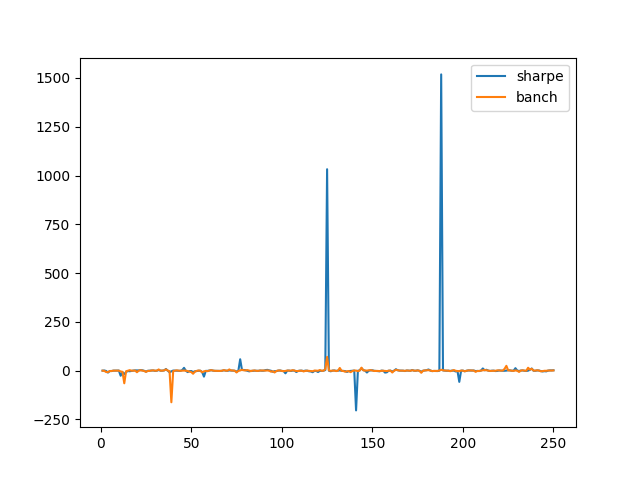
\includegraphics[clip, width=0.9\textwidth]{Graphics/TestFC3Dby10trainS.png} \caption{Sharpe Ratio of TEST 1}
\end{subfigure}%

\vspace{0.4cm}

It is better than both of using 10 days as a period to train and test and using 3 days as a period. Maybe training the model by using longer days as a period and test it by using shorter days as a period can get a better model.

\end{figure}

\newpage
\textbf{Using one pair of stocks’ 10 years data to train the model (n=3) using sharpe ratio as reward function}

We change the data we use. This time, we use the same one pair of stocks(AMAT \& CAJ) to train and test. We use 10 years data to train the model, and use the following one year of data to test it. And still use sharpe ratio as reward function.

\begin{figure}[H]
\begin{subfigure}{.5\textwidth}%
\centering
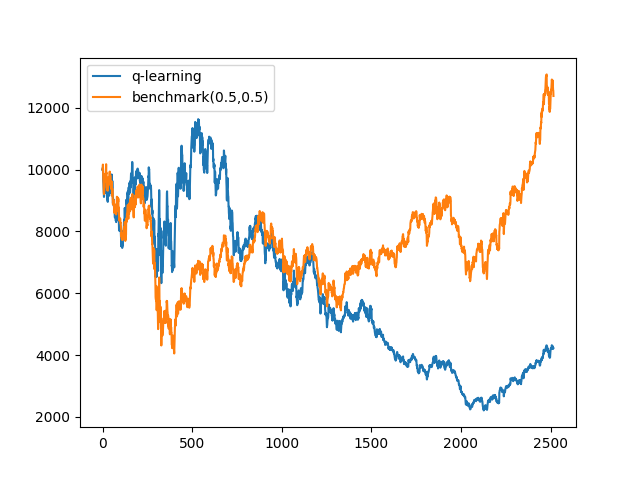
\includegraphics[clip, width=0.9\textwidth]{Graphics/NEW_TRY1.png} \caption{Training} 
\end{subfigure}%
\begin{subfigure}{.5\textwidth}%
\centering
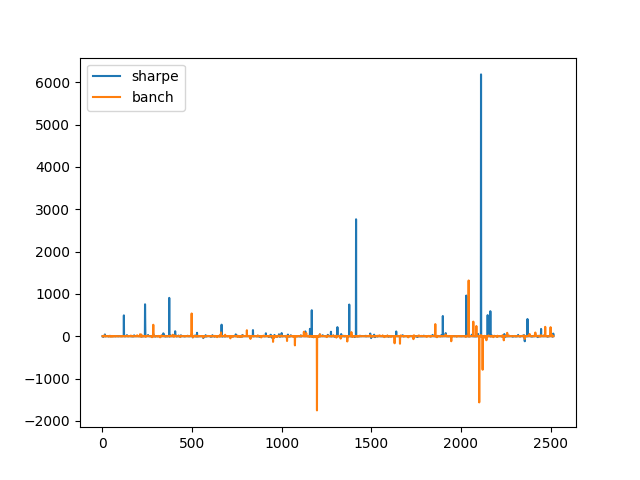
\includegraphics[clip, width=0.9\textwidth]{Graphics/NEW_TRY1S.png} \caption{Sharpe Ratio}
\end{subfigure}%
\vspace{0.4cm}
\begin{subfigure}{.5\textwidth}%
\centering
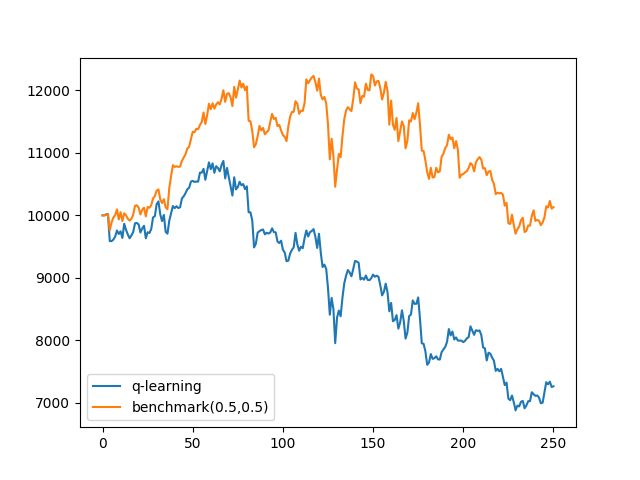
\includegraphics[clip, width=0.9\textwidth]{Graphics/NEW_TRY1TEST.png} \caption{Testing} 
\end{subfigure}%
\begin{subfigure}{.5\textwidth}%
\centering
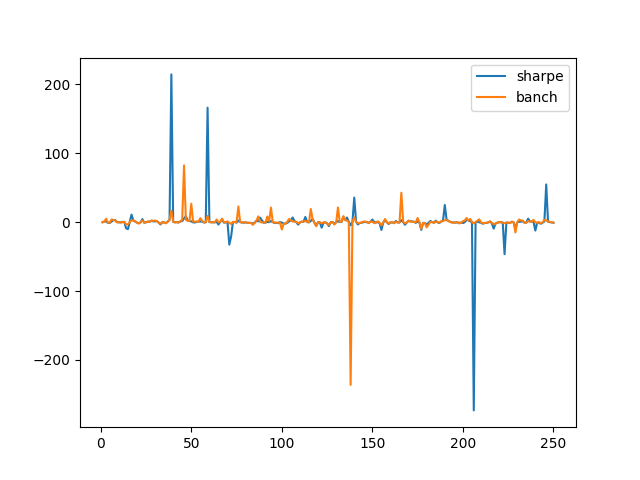
\includegraphics[clip, width=0.9\textwidth]{Graphics/NEW_TRY1TESTS.png} \caption{Sharpe Ratio}
\end{subfigure}%
\end{figure}

\newpage
Then we change to use total portfolio value as reward function
\begin{figure}[H]
\begin{subfigure}{.5\textwidth}%
\centering
\includegraphics[clip, width=0.9\textwidth]{Graphics/New_try_rewardpv.png} \caption{Training} 
\end{subfigure}%
\begin{subfigure}{.5\textwidth}%
\centering
\includegraphics[clip, width=0.9\textwidth]{Graphics/new_try_rewardpvS.png} \caption{Sharpe Ratio}
\end{subfigure}%
\vspace{0.4cm}
\begin{subfigure}{.5\textwidth}%
\centering
\includegraphics[clip, width=0.9\textwidth]{Graphics/NEW_TEST_REWARDPV.png} \caption{Testing} 
\end{subfigure}%
\begin{subfigure}{.5\textwidth}%
\centering
\includegraphics[clip, width=0.9\textwidth]{Graphics/REWARDPVS.png} \caption{Sharpe Ratio}
\end{subfigure}%
\end{figure}

\section{Deep Q-Network}

Q-learning has some obvious problems in our problem setting.
Firstly, to implement Q-learning we have to discretize the state, which is the stock price. However, if we discretize the stock price, the result we get will be inaccurate, which implies that the profit we get may not be optimized. Thus, it is necessary to find an alternative way that can handle the continuous state situation.

Secondly, it is impossible to find every Q-table value because there are tons of pairs of state and action in the project. Computer should be able to find action that fits our goal the most even when it runs into entirely new situation, but if Q-table values that computer finds are not enough computer will choose the action randomly. Thus, it is necessary to find another way that helps the computer find the right action without having to find out every single Q-table value directly.

To solve these two big problems, Deep Q Network is an appropriate method to solve them.

In our Deep Q Network algorithm, computer chooses action randomly with pre-determined probability, which is called ‘epsilon exploration’. It is mainly used in stochastic process like this situation where stock price changes randomly, because if without this epsilon exploration after one certain state happens computer choose the action depending on this specific state solely even though there are high probabilities the other states can happen as well. 
When neural networks are trained, we use mini-batch which picks items randomly in the memories which consists of plenty of pairs of state, action, reward, and next-state. In Q-learning, Q-table is updated with time and it is affected by time correlation. Unlike Q-learning, in Deep Q Network this algorithm called ‘Experience Replay’ is used to avoid correlation between each memory, especially with this kind of situation where time is related with, and it makes results better.     

In this project, fully connected layers, whose inputs are vectors, are used instead of convolutional neural networks, whose inputs are matrixes, because states in this project are price changes, which can be expressed more easily as vectors than matrixes. 

Relu and linear function are used as an activation function, Mean Squared Error function as a loss function, and Adam function as an optimizer. In terms of hyperparameters, we chose figures similar to those that are mainly used. 

\begin{figure}[H]
\begin{center}
\includegraphics[clip, width=0.4\textwidth]{Graphics/image1.png} \caption{Hyperparameters}
\end{center}
\end{figure}

In this Deep Q network algorithm, only two stocks, Applied Materials Inc. (AMAT) and Canon Inc. (CAJ), are used through all procedures.

We do training and testing separately, 10-years data which is from 08/03/2007 to 08/02/2017 is used for training and 1-year data which is from 08/03/2017 to 08/02/2018 is used for testing.  

The state is a vector that has 58 elements, each of which is price change between the day before and the day of each stock, because we use 30-days stock price for both stock as the state. 

The action is categorized into 11 options, which is the ratio between two stocks from 0 : 1 to 1 : 0, changing by 0.1 each. 
Naturally in this way the reward becomes the profit made by changing the action after a day.

It implies that computer chooses the ratio between two stocks which maximizes the profit by considering stock price changes in 30 days. 
The starting budget is 10,000\$ and transaction fee is 0.2\% of total transaction amount as same as Q-Learning, and we train it for 3,000, 5,000, and 50,000 episodes, respectively.

The graph shows the price change of AMAT and CAJ for 10-years of training period which is from 08/03/2007 to 08/02/2017.
After 10 years, AMAT price increases to 1.97 times, and CAJ price decreases to 0.63 times. 

\begin{figure}[H]
\begin{center}
\includegraphics[clip, width=0.6\textwidth]{Graphics/image3.png} \caption{Data}
\end{center}
\end{figure}

\textbf{Training}

\begin{figure}[H]
\begin{center}
\includegraphics[clip, width=0.8\textwidth]{Graphics/image8.png} \caption{Training 1 : With 3,000 episodes }
\end{center}
\end{figure}

Upper graph shows that the portfolio value of the last day after 10 years of training for every episode. Due to 0.2\% transaction fee, from the beginning to around 700th episode, the portfolio value stays less than 1,000. It suddenly passes 10,000 at 747th episode, and keeps increasing and  fluctuating continuously until about 2,500th episode. From 2,500th episode, it starts to surge dramatically, and at 2,921th episode the portfolio value peaks at 123,074.  

Lower graph shows the portfolio value as day passes at the final episode, which is 3,000th. A benchmark is the strategy that we allocate half of total budget to each stock every day. The total portfolio value of the benchmark is 12,433. Even though the final episode that this graph shows is not the episode that makes the profit the most, we can easily notice from this graph that Deep Q Network works much better than the benchmark.  

Deep Q Network works well in training, but one weakness is that fluctuation of the portfolio value for every episode is too widely as upper graph shows. We changed figures of hyperparameters to solve this problem, but nothing was effective. 

One thing to take a notice from the upper graph is from around 2,500th episode, there is a trend that the portfolio value increases steadily. Thus, we decided to run the same code with 5000 episodes.

\begin{figure}[H]
\begin{center}
\includegraphics[clip, width=0.8\textwidth]{Graphics/image10.png} \caption{Training 2 : With 5,000 episodes }
\end{center}
\end{figure}

As we guessed, in upper graph, after 3000th episode there are much more peaks than before. The maximum portfolio value is 520,438 with 4,602th episode. 

However, the weakness Deep Q Network has, fluctuating too much, was not solved at all. In the graph below, the result of 5000th episode is even worse, ending with only 23,321 portfolio value, comparing to 4,602th episode which ends with 520,438 portfolio value. 

Thus, hoping that it could be solved if the number of episodes increases a lot, thus we increased the number of episodes to 50,000.

\begin{figure}[H]
\begin{center}
\includegraphics[clip, width=0.8\textwidth]{Graphics/image9.png} \caption{Training 3 : With 50,000 episodes }
\end{center}
\end{figure}

The portfolio value of the last day still varies too much for every episode, but maximum portfolio value increased again. The maximum portfolio value is 914,586 which happened at 37,042th episode. It seems that a trend that maximum portfolio value increases as an episode goes stops, so we decided to stop training.  

Overall, training takes about 53 seconds per 100 episodes on average.

\begin{figure}[H]
\begin{center}
\includegraphics[clip, width=0.6\textwidth]{Graphics/image4.png} \caption{Data}
\end{center}
\end{figure}

For 1-year testing period, average of the prices of these two stocks do not change much, and after one year the average is almost same as the start point. 

We picked a model which has maximum portfolio value from each of three results. Thus, for 3,000 episodes, we picked 2,921th episode which has 123,074 portfolio value, for 5,000 episodes, we picked 4,602th episode which has 520,438 portfolio value, and for 50,000 episodes, we picked 37,042th episode which has 914,586 portfolio value. 

The benchmark is same with training, each stock has half of total budget for every single day.

\begin{figure}[H]
\begin{center}
\includegraphics[clip, width=0.6\textwidth]{Graphics/image6.png} \caption{Testing (3,000 episodes)}
\end{center}
\end{figure}

\begin{figure}[H]
\begin{center}
\includegraphics[clip, width=0.6\textwidth]{Graphics/image5.png} \caption{Testing (5,000 episodes)}
\end{center}
\end{figure}

\begin{figure}[H]
\begin{center}
\includegraphics[clip, width=0.6\textwidth]{Graphics/image7.png} \caption{Testing (50,000 episodes)}
\end{center}
\end{figure}

The portfolio value on the last day of a benchmark is 10,217, whereas the portfolio value for testing with the best result among 3,000 episodes is 9,217, a portfolio value for testing with the best result among 5,000 episodes is 6,511, and a portfolio value for testing with the best result among 5,000 episodes is 8,401. 

The point of these observation is that how good the result for training is has no relationship with how good the result for testing. Moreover, all three results have less portfolio value than the benchmark which just keeps the ratio with 50:50 for every single day. 

The chart below summarizes our results for both training and testing by Deep Q-Network. 

\begin{figure}[H]
\begin{center}
\includegraphics[clip, width=0.6\textwidth]{Graphics/image2.png} \caption{Comparasion}
\end{center}
\end{figure}



% Chapter 6
\ifthenelse{\boolean{@twoside}}{\myclearpage}{}
\chapter{Giving credit where credit is due}\label{Ch:GivingCredit}

The point was made in the Acknowledgments section of this Sample Report that it is important to credit others whose work you use---it is a matter of professional ethics and courtesy. 
In addition to acknowledgment of broad assistance or contributions that you put into the Acknowledgments, you may also need to reference more specific contributions elsewhere in your text.
Wherever a distinction is needed, make it clear which part of your work you have borrowed or adapted from others, and provide a reference to the source. 


\endinput


% Chapter 7
\ifthenelse{\boolean{@twoside}}{\myclearpage}{}
\chapter{Future Works}
\label{Ch:future}

There are some limitations of our research. Firstly, we just used two stocks to make portfolio. It would be better to build portfolio with various industry sectors. Secondly, we assumed that we can buy and sell stocks in non-integer form, which makes our model unrealistic. Thirdly, we defined the state only using the stock price, and we showed that it is hard to predict the stock price tendency by this way. Hence, for better portfolio model using stocks as assets, state should be defined on environmental factors such as market sentiment, average stock price of each industry sector. Or building portfolio model using various types of assets such as stocks, bonds, ETF funds considering the inflation, employment rate, market indexes would be better to derive more interesting conclusion. 


% Chapter 8 -- the Conclusion
\ifthenelse{\boolean{@twoside}}{\myclearpage}{}
\chapter{Final comments about polishing your report for publication}\label{Ch:Polishing}

Writing a good report is a serious challenge, requiring time and attention to details that are easily and often greatly underestimated by inexperienced writers.
So how does a good report acquire its final polish?

Your academic mentor will help guide your writing throughout your project.
He or she will be the first to review your report draft and edit it not only for style but also for technical correctness.
After you have satisfied your academic mentor with your draft, you will submit it to the RIPS program director for \emph{copy editing}, who will attend to matters of readability, grammar, and style.
After you submit your drafts for their review, it is likely they will return it to you with corrections, crossed out text, and possibly even suggestions
for overhauling whole parts of it. 
That is normal editing practice, and it is an expected part of the process of writing a professional-quality document.

Since your report is sponsored work, your sponsoring liaison should be given an opportunity to review it before its release.
But here's an important caution:  Don't submit a draft to your sponsor until 
\emph{after} it has been revised in compliance with suggestions from your academic mentor and the RIPS director.
It's good practice to give sponsors your most professional efforts---not your first drafts.
After you have satisfied the editing requirements of your academic mentor and the RIPS director, you should send your sponsor a \texttt{pdf} of a copy by email for review.
Your sponsor may suggest further changes.

\vspace{12pt}
\noindent You will facilitate the process of editing your report by submitting a single-sided printed copy for editing.
Double-sided is too hard to work with.
Although it is typical for copy editing to use double spacing of a manuscript to allow for editorial comments between lines, it is unnecessary for a RIPS report.
A table of {\em proofreader's marks} used by copy editors for mark-up, and used sometimes here at IPAM, is referenced in Appendix \ref{App:SourceLocation}.

After you have completed all the edits required by your academic mentor and the RIPS director, you can prepare final copies in two formats, respectively:
(1) a single-sided \texttt{pdf} as an electronic copy, which you can email to your sponsor, and 
(2) a slim double-sided copy for the final print version --- you can print this in the fatter single-sided format if your figures or text bleed through to the flip side of the page.
See Chapter \ref{Ch:ExtraAdvice} for a discussion of the special pagination requirements for double-sided copying.

Note that when you use \textsc{Adobe Reader} for printing your \texttt{pdf}, you are presented with options for {\em page scaling}.  You may have to play with this to get the  margins right.


\endinput


% Insert text in Table of Contents to highlight the appendix(es)
\addtocontents {toc}{\protect \contentsline {chapter}{APPENDIXES}{}}
\appendix
\ifthenelse{\boolean{@twoside}}{\myclearpage}{}
\chapter{Exchange Ratio}
\label{Exchange}
\section{Including Exchange Ratio}
In the later state of the project, we try to include the exchange ratio into our consideration. The application is that you can include two different countries' stock into the portfolio and settle at the end of the date with one of the stocks' currency in the portfolio. Since sometime due to the difference of public holiday and time-zone in different countries, we may face the situation that one country's stock market is working while the other one is not. When we face such situation, we will just skip that date in our training model.

The way we calculate the portfolio value is as follows
$$ pv_{t} = pv_{t-1} *[ (p_{t} / p_{t-1}) * w_{1}  + (q_{t} / q_{t-1}) * w_{2} * cv_{t}/cv_{t-1})]$$
the portfolio value will be in the currency you have chosen.
\endinput



\ifthenelse{\boolean{@twoside}}{\myclearpage}{}
\chapter{Where to find this sample RIPS report?}\label{App:SourceLocation}

Read-only {\LaTeX} source code for the RIPS Report Template, sample \textsc{Beamer} slide presentations, and other  {\LaTeX} supporting materials are available at,

\vspace{8pt}

\begin{verbatim}
Computer ->  IPAM RIPS FOLDER -> on the R Drive under under "Templates-etc"
\end{verbatim}

\noindent Your report will be ``copyedited'', i.e., edited for conformance to the RIPS \emph{House Style}.
For reference, a table of proofreader's marks that may be used for markup of your draft is included.
It was copied from {\em The Chicago Manual of Style, 16th ed}.
 (See original source at: \verb%www.chicagomanualofstyle.org/tools_proof.html%.)


\endinput

\ifthenelse{\boolean{@twoside}}{\myclearpage}{}
\chapter{Glossary}\label{Glossary}

\begin{table}[!h]  % Note override ("!") of normal placement algorithm to force placement on 1st page.
\begin{tabular}{ p{0.2\textwidth} p{0.75\textwidth} }

{\bf Page vs Leaf}:  &    In bookbinding, a trimmed sheet of paper bound in a book; each side of a leaf is a {\bf page}.\\  \\

{\bf Opening}:  &   The two pages you see when you open a book.  The right-hand {\bf page} is the {\bf recto}---and the left-hand page is the {\bf verso}.\\  \\


{\bf Recto}:  &  The front side of a {\bf leaf}; in a book or journal, a right-hand page.  To {\bf start recto} is to begin on a recto page, as any major section---e.g., title page, table of contents,  preface, chapter, appendix, bibliography---normally does. Contrast {\bf verso}.  \\  \\

{\bf Verso}:  &  The back side of a {\bf leaf}; the {\bf page} on the left-hand side of an {\bf opening}.\\  \\


{\bf Front matter}:  &  As applied to this report, the material that appears in the front of the document, including title page, the abstract, acknowledgments,  table of contents, list of figures, list of tables, usually numbered with lowercase roman numerals. RIPS reports initiate pagination with 1 in the front matter and proceed throughout with arabic numerals.
This variation of usage is allowed because modern typesetting permits easy re-pagination after pages have been added to the front matter, something not easily done---after completion of the main matter---when typesetting was done by hand.
 \\  \\


{\bf Main matter}: &  The main part of the document, including the appendixes.  {\bf Page} numbers start from 1 using arabic numerals if front matter is  enumerated using roman numerals. \\  \\

{\bf Back matter}: &  Material that appears at the back of the document, which in our report includes only the Bibliography. \\  \\

\end{tabular}
%\caption{A sample table used as a glossary.}
\end{table}

\endinput

\ifthenelse{\boolean{@twoside}}{\myclearpage}{}
\chapter{Abbreviations}\label{Abbreviations}

\noindent IPAM. Institute for Pure and Applied Mathematics.  An institute of the National Science  Foundation, located at UCLA.

\vspace{5pt}

\noindent RIPS.  Research in Industrial Projects for Students.  A regular summer program at IPAM, in which teams of undergraduate (or fresh graduate) students participate in sponsored team research projects.

\vspace{5pt}

\noindent UCLA.  The University of California at Los Angeles.

\vspace{5pt}




\endinput

% Add your bibliography to Contents
\ifthenelse{\boolean{@twoside}}{\myclearpage}{\newpage}
\addtocontents {toc}{\protect \contentsline {chapter}{REFERENCES}{}}
\addcontentsline{toc}{chapter}{Selected Bibliography Including Cited Works}  % Use the 'bibname' name here.  See below.

% Bibliography must come last.
\bibliographystyle{siam}     % Siam and Ieeetr bibliographic styles treat titles of articles in journals or collections correctly
\renewcommand\bibname{Selected Bibliography Including Cited Works}
\nocite{*}  % List ALL references in your references, not just the ones cited in the text.
% This scheme automatically alphabetizes the Bibliography.
\bibliography{AA-Bibliography/Biblio}

\end{document}
